% Options for packages loaded elsewhere
\PassOptionsToPackage{unicode}{hyperref}
\PassOptionsToPackage{hyphens}{url}
%
\documentclass[
  12pt]{article}
\usepackage{lmodern}
\usepackage{amssymb,amsmath}
\usepackage{ifxetex,ifluatex}
\ifnum 0\ifxetex 1\fi\ifluatex 1\fi=0 % if pdftex
  \usepackage[T1]{fontenc}
  \usepackage[utf8]{inputenc}
  \usepackage{textcomp} % provide euro and other symbols
\else % if luatex or xetex
  \usepackage{unicode-math}
  \defaultfontfeatures{Scale=MatchLowercase}
  \defaultfontfeatures[\rmfamily]{Ligatures=TeX,Scale=1}
\fi
% Use upquote if available, for straight quotes in verbatim environments
\IfFileExists{upquote.sty}{\usepackage{upquote}}{}
\IfFileExists{microtype.sty}{% use microtype if available
  \usepackage[]{microtype}
  \UseMicrotypeSet[protrusion]{basicmath} % disable protrusion for tt fonts
}{}
\makeatletter
\@ifundefined{KOMAClassName}{% if non-KOMA class
  \IfFileExists{parskip.sty}{%
    \usepackage{parskip}
  }{% else
    \setlength{\parindent}{0pt}
    \setlength{\parskip}{6pt plus 2pt minus 1pt}}
}{% if KOMA class
  \KOMAoptions{parskip=half}}
\makeatother
\usepackage{xcolor}
\IfFileExists{xurl.sty}{\usepackage{xurl}}{} % add URL line breaks if available
\IfFileExists{bookmark.sty}{\usepackage{bookmark}}{\usepackage{hyperref}}
\hypersetup{
  pdftitle={Trabajo Práctico 1},
  pdfauthor={Alcantara Fuentes, Victor Alan; Bocco, Alessio; Buscaglia, Florencia Paula; Ojeda, Rodrigo Nicolás},
  hidelinks,
  pdfcreator={LaTeX via pandoc}}
\urlstyle{same} % disable monospaced font for URLs
\usepackage[margin=1in]{geometry}
\usepackage{color}
\usepackage{fancyvrb}
\newcommand{\VerbBar}{|}
\newcommand{\VERB}{\Verb[commandchars=\\\{\}]}
\DefineVerbatimEnvironment{Highlighting}{Verbatim}{commandchars=\\\{\}}
% Add ',fontsize=\small' for more characters per line
\newenvironment{Shaded}{}{}
\newcommand{\AlertTok}[1]{\textcolor[rgb]{1.00,0.00,0.00}{\textbf{#1}}}
\newcommand{\AnnotationTok}[1]{\textcolor[rgb]{0.38,0.63,0.69}{\textbf{\textit{#1}}}}
\newcommand{\AttributeTok}[1]{\textcolor[rgb]{0.49,0.56,0.16}{#1}}
\newcommand{\BaseNTok}[1]{\textcolor[rgb]{0.25,0.63,0.44}{#1}}
\newcommand{\BuiltInTok}[1]{#1}
\newcommand{\CharTok}[1]{\textcolor[rgb]{0.25,0.44,0.63}{#1}}
\newcommand{\CommentTok}[1]{\textcolor[rgb]{0.38,0.63,0.69}{\textit{#1}}}
\newcommand{\CommentVarTok}[1]{\textcolor[rgb]{0.38,0.63,0.69}{\textbf{\textit{#1}}}}
\newcommand{\ConstantTok}[1]{\textcolor[rgb]{0.53,0.00,0.00}{#1}}
\newcommand{\ControlFlowTok}[1]{\textcolor[rgb]{0.00,0.44,0.13}{\textbf{#1}}}
\newcommand{\DataTypeTok}[1]{\textcolor[rgb]{0.56,0.13,0.00}{#1}}
\newcommand{\DecValTok}[1]{\textcolor[rgb]{0.25,0.63,0.44}{#1}}
\newcommand{\DocumentationTok}[1]{\textcolor[rgb]{0.73,0.13,0.13}{\textit{#1}}}
\newcommand{\ErrorTok}[1]{\textcolor[rgb]{1.00,0.00,0.00}{\textbf{#1}}}
\newcommand{\ExtensionTok}[1]{#1}
\newcommand{\FloatTok}[1]{\textcolor[rgb]{0.25,0.63,0.44}{#1}}
\newcommand{\FunctionTok}[1]{\textcolor[rgb]{0.02,0.16,0.49}{#1}}
\newcommand{\ImportTok}[1]{#1}
\newcommand{\InformationTok}[1]{\textcolor[rgb]{0.38,0.63,0.69}{\textbf{\textit{#1}}}}
\newcommand{\KeywordTok}[1]{\textcolor[rgb]{0.00,0.44,0.13}{\textbf{#1}}}
\newcommand{\NormalTok}[1]{#1}
\newcommand{\OperatorTok}[1]{\textcolor[rgb]{0.40,0.40,0.40}{#1}}
\newcommand{\OtherTok}[1]{\textcolor[rgb]{0.00,0.44,0.13}{#1}}
\newcommand{\PreprocessorTok}[1]{\textcolor[rgb]{0.74,0.48,0.00}{#1}}
\newcommand{\RegionMarkerTok}[1]{#1}
\newcommand{\SpecialCharTok}[1]{\textcolor[rgb]{0.25,0.44,0.63}{#1}}
\newcommand{\SpecialStringTok}[1]{\textcolor[rgb]{0.73,0.40,0.53}{#1}}
\newcommand{\StringTok}[1]{\textcolor[rgb]{0.25,0.44,0.63}{#1}}
\newcommand{\VariableTok}[1]{\textcolor[rgb]{0.10,0.09,0.49}{#1}}
\newcommand{\VerbatimStringTok}[1]{\textcolor[rgb]{0.25,0.44,0.63}{#1}}
\newcommand{\WarningTok}[1]{\textcolor[rgb]{0.38,0.63,0.69}{\textbf{\textit{#1}}}}
\usepackage{longtable,booktabs}
% Correct order of tables after \paragraph or \subparagraph
\usepackage{etoolbox}
\makeatletter
\patchcmd\longtable{\par}{\if@noskipsec\mbox{}\fi\par}{}{}
\makeatother
% Allow footnotes in longtable head/foot
\IfFileExists{footnotehyper.sty}{\usepackage{footnotehyper}}{\usepackage{footnote}}
\makesavenoteenv{longtable}
\usepackage{graphicx,grffile}
\makeatletter
\def\maxwidth{\ifdim\Gin@nat@width>\linewidth\linewidth\else\Gin@nat@width\fi}
\def\maxheight{\ifdim\Gin@nat@height>\textheight\textheight\else\Gin@nat@height\fi}
\makeatother
% Scale images if necessary, so that they will not overflow the page
% margins by default, and it is still possible to overwrite the defaults
% using explicit options in \includegraphics[width, height, ...]{}
\setkeys{Gin}{width=\maxwidth,height=\maxheight,keepaspectratio}
% Set default figure placement to htbp
\makeatletter
\def\fps@figure{htbp}
\makeatother
\setlength{\emergencystretch}{3em} % prevent overfull lines
\providecommand{\tightlist}{%
  \setlength{\itemsep}{0pt}\setlength{\parskip}{0pt}}
\setcounter{secnumdepth}{5}
\usepackage{booktabs}
\usepackage{colortbl}
\usepackage{setspace}
\usepackage{lineno}
\usepackage{float}
\usepackage{caption}
\usepackage{chngcntr}
\floatstyle{ruled}
\newfloat{codechunk}{htbp}{chk}
\floatname{codechunk}{Source Code}
\floatplacement{figure}{H}
\usepackage{booktabs}
\usepackage{siunitx}
\newcolumntype{d}{S[input-symbols = ()]}

\title{Trabajo Práctico 1}
\author{Alcantara Fuentes, Victor Alan \and Bocco, Alessio \and Buscaglia, Florencia Paula \and Ojeda, Rodrigo Nicolás}
\date{30 April, 2022}

\begin{document}
\maketitle

{
\setcounter{tocdepth}{2}
\tableofcontents
}
\hypertarget{introducciuxf3n}{%
\section{Introducción}\label{introducciuxf3n}}

El presente informe corresponde al Trabajo Práctico 1 de Métodos Estadísticos
Aplicados a los Negocios. El objetivo del mismo es la evaluación del efecto
de la comunicación entre compradores y vendedores en la plataforma eBay sobre
las probabilidades de venta.
El informe se estructura en tres secciones principales y un anexo. La primera consiste en un análisis exploratorio de los datos para la caracterización de las variables y la identificación de \emph{outliers}. Luego, el profiling finaliza con un análisis univariado y bivariado de las variables más pertinentes para el objetivo del estudio. La segunda sección contiene un análisis empírico del efecto de la introducción de nuevas metodologías de comunicación entre oferentes y demandantes. Por último, el reporte concluye con la aplicación de un modelo estadístico para la estimación del efecto de estas nuevas metodologías sobre las ventas. En el anexo se incluyen gráficos accesorios y una copia del código utilizado para la obtención de los resultados mostrados.

\hypertarget{exploraciuxf3n-del-dataset}{%
\section{Exploración del dataset}\label{exploraciuxf3n-del-dataset}}

\hypertarget{estructura-del-dataset}{%
\subsection{Estructura del dataset}\label{estructura-del-dataset}}

El dataset contiene 13 variables cuya descripción se detalla a continuación.

\begin{itemize}
\tightlist
\item
  date: fecha
\item
  itemid: id del producto
\item
  buyerid: id del comprador
\item
  itemsold: =1 si se vendió el producto, =0 en caso contrario
\item
  message: =1 si el comprador envió un mensaje, =0 en caso contrario
\item
  desktop: =1 si el comprador usó la versión desktop (A), =0 si usó la versión móvil (B)
\item
  post: =1 a partir del 23 de mayo de 2016, =0 antes de dicha fecha
\item
  category: categoría del producto en venta
\item
  condition: =1 si es nuevo, =0 si es usado
\item
  askingprice: precio ofrecido
\item
  holiday: =1 si es feriado, =0 en caso contrario
\item
  temp: temperatura
\item
  precipitation: precipitaciones
\end{itemize}

\hypertarget{tipos-de-variables}{%
\subsubsection{Tipos de variables}\label{tipos-de-variables}}

La Tabla \ref{tab:tipos-variable} muestra los tipos de variables presentes en el dataset. Para cada una de ellas se muestra el tipo de dato y la cantidad de faltantes y valores únicos.

\begin{table}[H]

\caption{\label{tab:tipos-variable}Tipos de variables presentes.}
\centering
\resizebox{\linewidth}{!}{
\begin{tabular}[t]{llrrrr}
\toprule
Variables & Tipo & Faltantes (N) & Faltantes (\%) & Único (N) & Único (tasa)\\
\midrule
\cellcolor{gray!6}{date} & \cellcolor{gray!6}{Date} & \cellcolor{gray!6}{0} & \cellcolor{gray!6}{0} & \cellcolor{gray!6}{56} & \cellcolor{gray!6}{0.000280}\\
itemid & numeric & 0 & 0 & 5 & 0.000025\\
\cellcolor{gray!6}{buyerid} & \cellcolor{gray!6}{numeric} & \cellcolor{gray!6}{0} & \cellcolor{gray!6}{0} & \cellcolor{gray!6}{493} & \cellcolor{gray!6}{0.002465}\\
itemsold & numeric & 0 & 0 & 2 & 0.000010\\
\cellcolor{gray!6}{message} & \cellcolor{gray!6}{numeric} & \cellcolor{gray!6}{0} & \cellcolor{gray!6}{0} & \cellcolor{gray!6}{2} & \cellcolor{gray!6}{0.000010}\\
\addlinespace
desktop & numeric & 0 & 0 & 2 & 0.000010\\
\cellcolor{gray!6}{post} & \cellcolor{gray!6}{numeric} & \cellcolor{gray!6}{0} & \cellcolor{gray!6}{0} & \cellcolor{gray!6}{2} & \cellcolor{gray!6}{0.000010}\\
category & character & 0 & 0 & 5 & 0.000025\\
\cellcolor{gray!6}{condition} & \cellcolor{gray!6}{numeric} & \cellcolor{gray!6}{0} & \cellcolor{gray!6}{0} & \cellcolor{gray!6}{2} & \cellcolor{gray!6}{0.000010}\\
askingprice & numeric & 0 & 0 & 36798 & 0.183990\\
\addlinespace
\cellcolor{gray!6}{holiday} & \cellcolor{gray!6}{numeric} & \cellcolor{gray!6}{0} & \cellcolor{gray!6}{0} & \cellcolor{gray!6}{2} & \cellcolor{gray!6}{0.000010}\\
temp & numeric & 0 & 0 & 25 & 0.000125\\
\cellcolor{gray!6}{precipitation} & \cellcolor{gray!6}{numeric} & \cellcolor{gray!6}{0} & \cellcolor{gray!6}{0} & \cellcolor{gray!6}{14} & \cellcolor{gray!6}{0.000070}\\
\bottomrule
\end{tabular}}
\end{table}

Del análisis exploratorio realizado, se observaron las siguientes situaciones:

\begin{itemize}
\tightlist
\item
  Tipos de variables:

  \begin{itemize}
  \tightlist
  \item
    Fecha: Date
  \item
    Categórica: cateogry
  \item
    Cuantitativas:

    \begin{itemize}
    \tightlist
    \item
      Continuas: itemid, buyerid, askingprice, temp, precipitation
    \item
      Discretas: itemsold, message, desktop, post, condition, holiday
    \end{itemize}
  \end{itemize}
\item
  Ninguna variable cuenta con valores faltantes.
\item
  Si bien en la Tabla \ref{tab:tipos-variable} algunas de las variables cuantitativas discretas se muestran como numéricas, en realidad se trata de variables dicotómicas que expresan la ausencia o presencia de determinada cuestión.
\end{itemize}

\hypertarget{variables-cuantitativas}{%
\subsubsection{Variables cuantitativas}\label{variables-cuantitativas}}

Dentro de las variables cuantitativas, la Tabla \ref{tab:variable-numerica} muestra las principales medidas de resumen que caracterizan a cada una de ellas.

\begin{table}[H]

\caption{\label{tab:variable-numerica}Diagnóstico variables cuantitativas}
\centering
\resizebox{\linewidth}{!}{
\begin{tabular}[t]{lrrrrrrrr}
\toprule
variables & min & Q1 & mean & median & Q3 & max & zero & minus\\
\midrule
\cellcolor{gray!6}{itemid} & \cellcolor{gray!6}{1200000000.00} & \cellcolor{gray!6}{3400000000.00} & \cellcolor{gray!6}{5417668500.000000} & \cellcolor{gray!6}{5600000000.00} & \cellcolor{gray!6}{7800000000.00} & \cellcolor{gray!6}{9100000000.00} & \cellcolor{gray!6}{0} & \cellcolor{gray!6}{0}\\
buyerid & 7384.00 & 250000000.00 & 500117278.912840 & 500000000.00 & 750000000.00 & 1000000000.00 & 0 & 0\\
\cellcolor{gray!6}{itemsold} & \cellcolor{gray!6}{0.00} & \cellcolor{gray!6}{0.00} & \cellcolor{gray!6}{0.479980} & \cellcolor{gray!6}{0.00} & \cellcolor{gray!6}{1.00} & \cellcolor{gray!6}{1.00} & \cellcolor{gray!6}{104004} & \cellcolor{gray!6}{0}\\
message & 0.00 & 0.00 & 0.070305 & 0.00 & 0.00 & 1.00 & 185939 & 0\\
\cellcolor{gray!6}{desktop} & \cellcolor{gray!6}{0.00} & \cellcolor{gray!6}{0.00} & \cellcolor{gray!6}{0.551970} & \cellcolor{gray!6}{1.00} & \cellcolor{gray!6}{1.00} & \cellcolor{gray!6}{1.00} & \cellcolor{gray!6}{89606} & \cellcolor{gray!6}{0}\\
\addlinespace
post & 0.00 & 0.00 & 0.500105 & 1.00 & 1.00 & 1.00 & 99979 & 0\\
\cellcolor{gray!6}{condition} & \cellcolor{gray!6}{0.00} & \cellcolor{gray!6}{0.00} & \cellcolor{gray!6}{0.425750} & \cellcolor{gray!6}{0.00} & \cellcolor{gray!6}{1.00} & \cellcolor{gray!6}{1.00} & \cellcolor{gray!6}{114850} & \cellcolor{gray!6}{0}\\
askingprice & 2.53 & 5.06 & 92.725363 & 16.24 & 66.09 & 5874.36 & 0 & 0\\
\cellcolor{gray!6}{holiday} & \cellcolor{gray!6}{0.00} & \cellcolor{gray!6}{0.00} & \cellcolor{gray!6}{0.090485} & \cellcolor{gray!6}{0.00} & \cellcolor{gray!6}{0.00} & \cellcolor{gray!6}{1.00} & \cellcolor{gray!6}{181903} & \cellcolor{gray!6}{0}\\
temp & 5.50 & 12.00 & 14.811587 & 16.50 & 18.00 & 22.50 & 0 & 0\\
\addlinespace
\cellcolor{gray!6}{precipitation} & \cellcolor{gray!6}{0.00} & \cellcolor{gray!6}{0.00} & \cellcolor{gray!6}{3.224925} & \cellcolor{gray!6}{0.00} & \cellcolor{gray!6}{5.00} & \cellcolor{gray!6}{45.00} & \cellcolor{gray!6}{110833} & \cellcolor{gray!6}{0}\\
\bottomrule
\end{tabular}}
\end{table}

A partir de la Tabla se observa lo siguiente:

\begin{itemize}
\tightlist
\item
  itemdid y buyerid: corresponden a indentificadores unívocos de uso interno y carecen de valor para el presente estudio.
\item
  Se confirma el carácter dictómico de las variables identificadas en el apartado anterior.
\item
  La variable askingprice exhibe un fuerte sesgo a izquierda dado que la media es muy superior a la mediana. También tiene una importante disperión dada la diferencia entre el limite superior del intervalo intercuartílico y el máximo. No presenta valores negativos ni nulos por lo que es consistente con su significado. * Las variables meteorológicas \emph{temp} y \emph{precipitation} muestran un comportamiento consistente con lo que se esperaría para variables de este tipo.
\end{itemize}

\hypertarget{variables-categuxf3ricas}{%
\subsubsection{Variables categóricas}\label{variables-categuxf3ricas}}

La Tabla \ref{tab:variable-categorica} muestra una tabla de contigencia con las principales métricas que describen cada categoría de la variable \emph{category}

\begin{table}[H]

\caption{\label{tab:variable-categorica}Diagnóstico variables categóricas}
\centering
\resizebox{\linewidth}{!}{
\begin{tabular}[t]{llrrrr}
\toprule
Variable & Clases & N & Freq & Ratio & Ranking\\
\midrule
\cellcolor{gray!6}{category} & \cellcolor{gray!6}{Clothing, Shoes, \& Accessories} & \cellcolor{gray!6}{200000} & \cellcolor{gray!6}{40206} & \cellcolor{gray!6}{20.1030} & \cellcolor{gray!6}{1}\\
category & Toys \& Hobbies & 200000 & 40127 & 20.0635 & 2\\
\cellcolor{gray!6}{category} & \cellcolor{gray!6}{Jewelry \& Watches} & \cellcolor{gray!6}{200000} & \cellcolor{gray!6}{40029} & \cellcolor{gray!6}{20.0145} & \cellcolor{gray!6}{3}\\
category & Books & 200000 & 39841 & 19.9205 & 4\\
\cellcolor{gray!6}{category} & \cellcolor{gray!6}{Computer/Tablets \& Networking} & \cellcolor{gray!6}{200000} & \cellcolor{gray!6}{39797} & \cellcolor{gray!6}{19.8985} & \cellcolor{gray!6}{5}\\
\bottomrule
\end{tabular}}
\end{table}

Las cinco clases tienen una cantidad de observaciones muy similar, con una frecuencia en torno al 20\%.

\hypertarget{muestra-del-dataset}{%
\subsubsection{Muestra del dataset}\label{muestra-del-dataset}}

A continuación de muestra la Tabla \ref{tab:muestra-dataset} dónde se observan las 5 primeras filas del dataset.

\begin{table}[H]

\caption{\label{tab:muestra-dataset}Muestra del dataset}
\centering
\resizebox{\linewidth}{!}{
\begin{tabular}[t]{lrrrrrrlrrrrr}
\toprule
date & itemid & buyerid & itemsold & message & desktop & post & category & condition & askingprice & holiday & temp & precipitation\\
\midrule
\cellcolor{gray!6}{2016-04-25} & \cellcolor{gray!6}{9100000000} & \cellcolor{gray!6}{200000000} & \cellcolor{gray!6}{0} & \cellcolor{gray!6}{0} & \cellcolor{gray!6}{1} & \cellcolor{gray!6}{0} & \cellcolor{gray!6}{Computer/Tablets \& Networking} & \cellcolor{gray!6}{1} & \cellcolor{gray!6}{4.93} & \cellcolor{gray!6}{0} & \cellcolor{gray!6}{5.5} & \cellcolor{gray!6}{11}\\
2016-04-25 & 9100000000 & 360000000 & 0 & 0 & 1 & 0 & Computer/Tablets \& Networking & 1 & 15.23 & 0 & 5.5 & 11\\
\cellcolor{gray!6}{2016-04-25} & \cellcolor{gray!6}{7800000000} & \cellcolor{gray!6}{81000000} & \cellcolor{gray!6}{1} & \cellcolor{gray!6}{0} & \cellcolor{gray!6}{1} & \cellcolor{gray!6}{0} & \cellcolor{gray!6}{Clothing, Shoes, \& Accessories} & \cellcolor{gray!6}{1} & \cellcolor{gray!6}{33.81} & \cellcolor{gray!6}{0} & \cellcolor{gray!6}{5.5} & \cellcolor{gray!6}{11}\\
2016-04-25 & 5600000000 & 160000000 & 0 & 0 & 1 & 0 & Jewelry \& Watches & 0 & 51.79 & 0 & 5.5 & 11\\
\cellcolor{gray!6}{2016-04-25} & \cellcolor{gray!6}{7800000000} & \cellcolor{gray!6}{27000000} & \cellcolor{gray!6}{0} & \cellcolor{gray!6}{0} & \cellcolor{gray!6}{1} & \cellcolor{gray!6}{0} & \cellcolor{gray!6}{Clothing, Shoes, \& Accessories} & \cellcolor{gray!6}{0} & \cellcolor{gray!6}{10.07} & \cellcolor{gray!6}{0} & \cellcolor{gray!6}{5.5} & \cellcolor{gray!6}{11}\\
\addlinespace
2016-04-25 & 5600000000 & 930000000 & 0 & 0 & 1 & 0 & Jewelry \& Watches & 1 & 30.91 & 0 & 5.5 & 11\\
\bottomrule
\end{tabular}}
\end{table}

A partir de éste primer análisis exploratorio y en función del objetivo del estudio se seleccionaron las variables \emph{itemsold}, \emph{desktop}, \emph{post}, \emph{condition}, \emph{holiday}, \emph{temp} y \emph{precipitation}. Sobre las mencionadas variables se mostrará a continuación un análisis uni y bivariado y se evaluará la presencia de outliers en las variables cuantitativas seleccionadas.

\hypertarget{anuxe1lisis-univariado-y-bivariado}{%
\subsection{Análisis univariado y bivariado}\label{anuxe1lisis-univariado-y-bivariado}}

\hypertarget{cantidad-de-ventas-por-plataforma}{%
\subsubsection{Cantidad de ventas por plataforma}\label{cantidad-de-ventas-por-plataforma}}

La Figura \ref{fig:ventas-plataforma} muestra la cantidad de ventas por tipo de plataforma. En el panel izquierdo se muestran la cantidad de operaciones totales y en el derecha la cantidad de ventas concretadas. Se observa una distribución bastante pareja entre ambas, con un 45\% de las ventas en la versión móvil y un 55\% en la versión de escritorio.

\begin{figure}

{\centering \includegraphics{/Users/alessiobocco/Documents/Maestria/Maestría Di Tella/Métodos Estadísticos Aplicados a Negocios/Trabajo Practico/trabajo_practico_files/figure-latex/ventas-plataforma-1} 

}

\caption{Ventas por tipo de plataforma.}\label{fig:ventas-plataforma}
\end{figure}

\hypertarget{cantidad-de-ventas-por-momento-de-compra}{%
\subsubsection{Cantidad de ventas por momento de compra}\label{cantidad-de-ventas-por-momento-de-compra}}

La Figura \ref{fig:ventas-momento} muestra la cantidad de operaciones antes y después del 23 de mayo de 2016, momento en que se permitió interacción entre compradores y vendedores. En el panel izquierdo se muestran la cantidad de operaciones totales y en el derecha la cantidad de ventas concretadas. se observa que la cantidad de operaciones total fue la misma para ambos momentos pero hubo un ligero aumento en las ventas concretadas a partir de la posibilidad de interacción.

\begin{figure}

{\centering \includegraphics{/Users/alessiobocco/Documents/Maestria/Maestría Di Tella/Métodos Estadísticos Aplicados a Negocios/Trabajo Practico/trabajo_practico_files/figure-latex/ventas-momento-1} 

}

\caption{Ventas anteriores y posteriores al cambio en la plataforma.}\label{fig:ventas-momento}
\end{figure}

\hypertarget{cantidad-de-ventas-por-condiciuxf3n-del-producto}{%
\subsubsection{Cantidad de ventas por condición del producto}\label{cantidad-de-ventas-por-condiciuxf3n-del-producto}}

La Figura \ref{fig:ventas-condicion} muestra la cantidad de operaciones (izquierda) y ventas (derecha) según la condición del producto, es decir, si se trata de un producto nuevo o usado.

\begin{figure}

{\centering \includegraphics{/Users/alessiobocco/Documents/Maestria/Maestría Di Tella/Métodos Estadísticos Aplicados a Negocios/Trabajo Practico/trabajo_practico_files/figure-latex/ventas-condicion-1} 

}

\caption{Ventas según la condición del producto.}\label{fig:ventas-condicion}
\end{figure}

\hypertarget{efecto-de-las-condiciones-climuxe1ticas}{%
\subsubsection{Efecto de las condiciones climáticas}\label{efecto-de-las-condiciones-climuxe1ticas}}

La Figura \ref{fig:ventas-temperatura} muestra la cantidad de ventas y operaciones por percentil de temperatura. Es decir, se dividió la variable \emph{temp} en 5 percentiles iguales y se contaron la cantidad de operaciones (izquierda) y ventas (derecha) que se llevaron a cabo en cada uno de ellos.

\begin{figure}

{\centering \includegraphics{/Users/alessiobocco/Documents/Maestria/Maestría Di Tella/Métodos Estadísticos Aplicados a Negocios/Trabajo Practico/trabajo_practico_files/figure-latex/ventas-temperatura-1} 

}

\caption{Ventas según el percentil de temperatura.}\label{fig:ventas-temperatura}
\end{figure}

En la Figura no se observan diferencias significativas entre clases tanto para operaciones como para ventas concretadas.

\hypertarget{precipitaciuxf3n}{%
\subsubsection{Precipitación}\label{precipitaciuxf3n}}

La Figura \ref{fig:ventas-precipitacion} muestra la cantidad de ventas y operaciones por tipo de día. La Organización Meteorológica Mundial (OMM) clasifica a los días en lluviosos o secos si la precipitación acumulada diaria es superior a 0.5 mm. Si bien no se conoce la unidad de medida de la variable se asume que está expresada en el sistema métrico. Luego, se contaron la cantidad de operaciones (izquierda) y ventas (derecha) que se llevaron a cabo en cada uno de ellos.

\begin{figure}

{\centering \includegraphics{/Users/alessiobocco/Documents/Maestria/Maestría Di Tella/Métodos Estadísticos Aplicados a Negocios/Trabajo Practico/trabajo_practico_files/figure-latex/ventas-precipitacion-1} 

}

\caption{Ventas según el tipo de día.}\label{fig:ventas-precipitacion}
\end{figure}

En la Figura no se observan diferencias significativas entre clases tanto para operaciones como para ventas concretadas.

\hypertarget{anuxe1lisis-de-outliers}{%
\subsection{Análisis de outliers}\label{anuxe1lisis-de-outliers}}

Los outliers se identificaron para las variables cuantitativas continuas. La fórmula utilizada para fue la por defecto en R para el diagrama de cajas. La misma se detalla a continuación.

\begin{Shaded}
\begin{Highlighting}[]
\CommentTok{# Outliers inferiores}
\KeywordTok{max}\NormalTok{(}\KeywordTok{min}\NormalTok{(x), Q1 }\OperatorTok{-}\StringTok{ }\NormalTok{(}\KeywordTok{IQR}\NormalTok{(x)}\OperatorTok{*}\FloatTok{1.5}\NormalTok{))}
\CommentTok{# Outliers superiores}
\KeywordTok{min}\NormalTok{(}\KeywordTok{max}\NormalTok{(x), Q3 }\OperatorTok{+}\StringTok{ }\NormalTok{(}\KeywordTok{IQR}\NormalTok{(x)}\OperatorTok{*}\FloatTok{1.5}\NormalTok{)) }
\end{Highlighting}
\end{Shaded}

La Tabla @ref(tab:out\_tabla) muestra los resultados del análisis. Sólo se detectaron valores anómalos en \emph{askingprice} pero dado que nor formará parte del análisis no se hizo más hincapié en ellos.

\begin{table}[H]
\centering
\resizebox{\linewidth}{!}{
\begin{tabular}{lrrrrr}
\toprule
variables & outliers\_cnt & outliers\_ratio & outliers\_mean & with\_mean & without\_mean\\
\midrule
\cellcolor{gray!6}{askingprice} & \cellcolor{gray!6}{28048} & \cellcolor{gray!6}{14.024} & \cellcolor{gray!6}{496.73982} & \cellcolor{gray!6}{92.725363} & \cellcolor{gray!6}{26.824429}\\
temp & 0 & 0.000 & NaN & 14.811587 & 14.811587\\
\cellcolor{gray!6}{precipitation} & \cellcolor{gray!6}{10748} & \cellcolor{gray!6}{5.374} & \cellcolor{gray!6}{28.84518} & \cellcolor{gray!6}{3.224925} & \cellcolor{gray!6}{1.769899}\\
\bottomrule
\end{tabular}}
\end{table}

Con respecto a la precipitación, esta variable tiene un comportamiento especial cuando se trata de valores diarios. Existen una gran cantidad de ceros por lo que es muy frecuente la identificación de outliers cuando en realidad no lo son. El análisis de valores extremos de lluvia está fuera del alcance del presente pero se muestra en la Figura \ref{fig:precip-outlier} la distribución de la variable considerando los valores anómalos en el panel superior y luego de su eliminación en el inferior.

\begin{figure}

{\centering 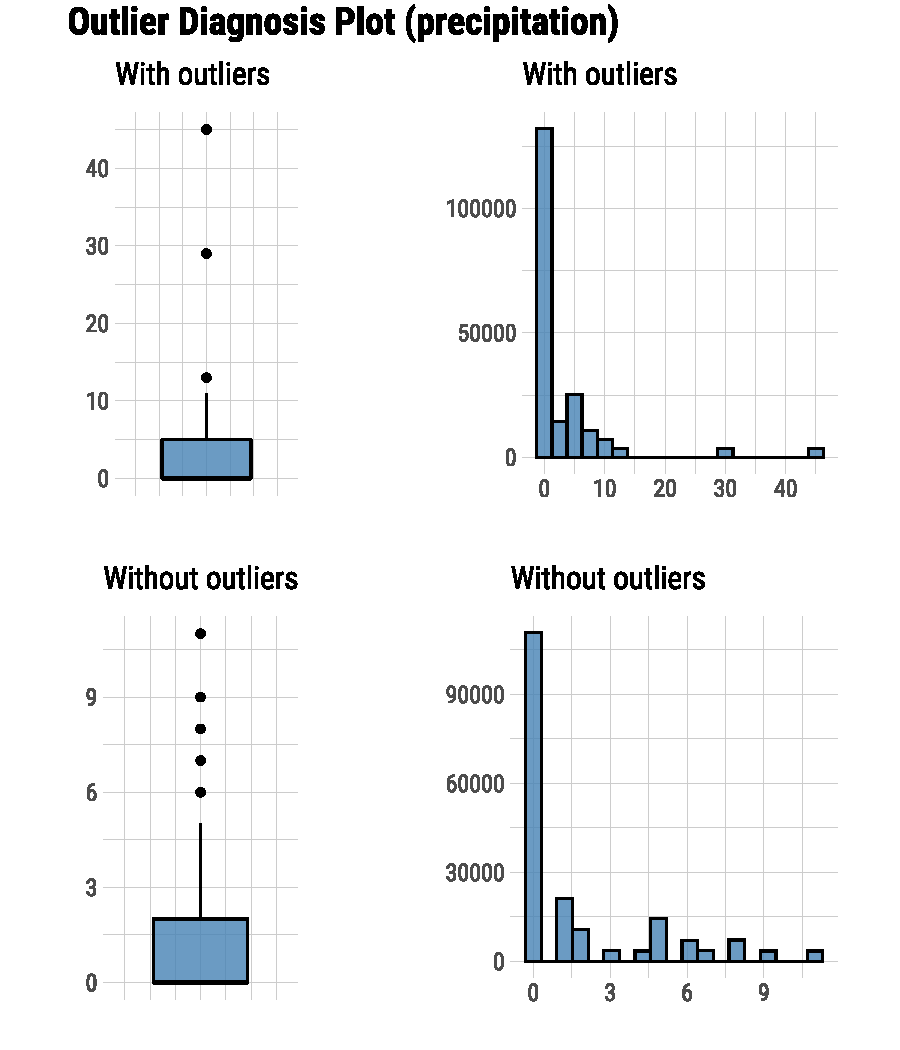
\includegraphics{/Users/alessiobocco/Documents/Maestria/Maestría Di Tella/Métodos Estadísticos Aplicados a Negocios/Trabajo Practico/trabajo_practico_files/figure-latex/precip-outlier-1} 

}

\caption{Outliers de la variable precipitación}\label{fig:precip-outlier}
\end{figure}

\hypertarget{anuxe1lisis-de-ventas}{%
\section{Análisis de ventas}\label{anuxe1lisis-de-ventas}}

En la presente sección comienza el análisis del impacto en la ventas de la nueva estrategia de comunicación. En la \ref{fig:intervalo-confianza} muestra la proporción de ventas para las dos plataformas (Escritorio y Móvil) y antes y después de permitir la interacción. El punto de la Figura corresponde a la proporción de ventas en cada combinación de plataforma/momento y las barras al intervalo de confianza del 95\% (percentiles).

\begin{figure}

{\centering \includegraphics{/Users/alessiobocco/Documents/Maestria/Maestría Di Tella/Métodos Estadísticos Aplicados a Negocios/Trabajo Practico/trabajo_practico_files/figure-latex/intervalo-confianza-1} 

}

\caption{Proporción de las ventas por plataforma y momento de observación.}\label{fig:intervalo-confianza}
\end{figure}

Del gráfico obtenido para los intervalos de confianza se observa la existencia de solapamiento en particular entre la proporción de ventas de la versión Móvil (después del 23.05) y la proporción de ventas de la versión Desktop (antes del 23.05). Tal situación podría generar ruido en la base de datos y no permitir que se pueda diferenciar el real impacto de la variable `post' en el incremento de la probabilidad de que se realice una venta cuando el comprador y vendedor se comuniquen.

Luego de conocer las proporciones con sus respectivos intervalos de confianza se realizó una prueba de proporciones para conocer si el cambio impulsó la cantidad de ventas en la versión Desktop. La \ref{tab:salida-prueba} muestra los resultados de dicha prueba.

\begin{table}[H]

\caption{\label{tab:salida-prueba}Resúmen de la prueba de hipótesis.}
\centering
\resizebox{\linewidth}{!}{
\begin{tabular}[t]{rrrll}
\toprule
Media estimada & Estadístico & p.valor & método & Hipótesis alternativa\\
\midrule
\cellcolor{gray!6}{0.4878028} & \cellcolor{gray!6}{13.66092} & \cellcolor{gray!6}{0.9998905} & \cellcolor{gray!6}{1-sample proportions test without continuity correction} & \cellcolor{gray!6}{greater}\\
\bottomrule
\end{tabular}}
\end{table}

De la prueba de hipótesis realizada se verificó que al 95\% de confianza no hay evidencia para rechazar la hipótesis nula de que la proporción de ventas de productos nuevos en la versión Desktop después del 23 de mayo de 2016 no sea superior al 50\%, por lo que se puede afirmar que tal proporción no es superior al 50\%.

\hypertarget{potencia-de-la-prueba}{%
\subsubsection{Potencia de la prueba}\label{potencia-de-la-prueba}}

La \ref{fig:potencia-prueba} muestra la potencia de la prueba anterior para distintos tamaños de muestra utilizando un valor de \(\alpha\) de 0.05.

\begin{figure}

{\centering \includegraphics{/Users/alessiobocco/Documents/Maestria/Maestría Di Tella/Métodos Estadísticos Aplicados a Negocios/Trabajo Practico/trabajo_practico_files/figure-latex/potencia-prueba-1} 

}

\caption{Potencia de la prueba de hipótesis para distintos tamaños muestrales.}\label{fig:potencia-prueba}
\end{figure}

Se observa el rápido crecimiento de la curva al aumentar el tamaño muestral en sintonía con la que se esperaría en base a la teoría.

\hypertarget{modelos-de-regresiuxf3n}{%
\subsection{Modelos de regresión}\label{modelos-de-regresiuxf3n}}

En la presente sección se muestran distintos modelos para explicar el efecto de distintas variables sobre la probabilidad de que se concrete una compra. Para ello se utilizará un modelo de probabilidad lineal (LPM, por sus siglas en inglés). Estos modelos son especialmente interesantes para explorar los efectos marginales sobre la variable de interés. A continuación se presentan distintos modelos con un grado creciente de complejidad.

\hypertarget{modelo-buxe1sico}{%
\subsubsection{Modelo básico}\label{modelo-buxe1sico}}

La ecuación del modelo básico se muestra en la ecuación 1. Las principales variables del modelo son \emph{desktop} y \emph{post}.

\begin{equation}
\operatorname{itemsold} = \beta_{0} + \beta_{1}(\operatorname{desktop}) + \beta_{2}(\operatorname{post}) + \beta_{3}(\operatorname{desktop} \times \operatorname{post}) + \epsilon
\end{equation}

Los resultados del modelo de muestran en la tabla siguiente.

\begin{table}[H]
\centering
\begin{tabular}[t]{lc}
\toprule
  & Model 1\\
\midrule
(Intercept) & \num{0.448}\\
 & {}[\num{0.443}, \num{0.453}]\\
 & s.e. = \num{0.002}\\
 & t = \num{190.730}\\
 & p = \vphantom{3} \num{0.000}\\
desktop & \num{0.020}\\
 & {}[\num{0.014}, \num{0.026}]\\
 & s.e. = \vphantom{1} \num{0.003}\\
 & t = \num{6.272}\\
 & p = \vphantom{2} \num{0.000}\\
post & \num{0.022}\\
 & {}[\num{0.016}, \num{0.029}]\\
 & s.e. = \num{0.003}\\
 & t = \num{6.679}\\
 & p = \vphantom{1} \num{0.000}\\
desktop × post & \num{0.036}\\
 & {}[\num{0.027}, \num{0.045}]\\
 & s.e. = \num{0.004}\\
 & t = \num{8.000}\\
 & p = \num{0.000}\\
\midrule
Num.Obs. & \num{200000}\\
R2 & \num{0.004}\\
R2 Adj. & \num{0.003}\\
AIC & \num{289303.1}\\
BIC & \num{289354.2}\\
Log.Lik. & \num{-144646.570}\\
F & \num{234.527}\\
Std.Errors & Robust\\
\bottomrule
\end{tabular}
\end{table}

Mientras que el modelo ajustado se muestra en la ecuación 2.

\begin{equation}
\begin{aligned}
\operatorname{\widehat{itemsold}} &= 0.448 + 0.02(\operatorname{desktop}) + 0.022(\operatorname{post}) + 0.036(\operatorname{desktop} \times \operatorname{post})
\end{aligned}
\end{equation}

De la estimación realizada, se observa que, manteniendo lo demás constante, el hecho de utilizar la versión Desktop de la plataforma incrementa la probabilidad de que se realice una venta en 1.98 puntos porcentuales (\(\beta_1\)); el hecho de que se esté en un momento a partir del 23.05.2016, incrementa la probabilidad de que se realice una venta en 2.22 puntos porcentuales (\(\beta_2\)); y el hecho de que se utilice la versión Desktop de la plataforma y a la vez se esté en un momento a partir del 23.05.2016, incrementa la probabilidad de que se realice una venta en 3.58 puntos porcentuales \(\beta_3\)).
Por otro lado, el hecho que el comprador y vendedor tengan la probabilidad de comunicarse incrementa la probabilidad de que se concrete una venta en 7.79 puntos porcentuales (\(\beta_1\) + \(\beta_2\) + \(\beta_3\)).

Además del análisis del modelo básico original se realizaron 1000 replicaciones del mismo para evaluar la estabilidad de los coeficientes. Los resultados del bootstrap se muestra en la Figura \ref{fig:boot-modelo-basico}.

\begin{figure}

{\centering \includegraphics{/Users/alessiobocco/Documents/Maestria/Maestría Di Tella/Métodos Estadísticos Aplicados a Negocios/Trabajo Practico/trabajo_practico_files/figure-latex/boot-modelo-basico-1} 

}

\caption{Coeficientes a partir del remuestreo del modelo de regresión básico.}\label{fig:boot-modelo-basico}
\end{figure}

En la Figura se muestra la densidad de los coeficientes en negro mientras que las barras rojas corresponden al intervalo de confianza del 95\% calculado a partir de los percentiles.

\hypertarget{modelo-buxe1sico-condiciuxf3n-del-producto}{%
\subsubsection{Modelo básico + condición del producto}\label{modelo-buxe1sico-condiciuxf3n-del-producto}}

La ecuación del modelo básico se muestra en la ecuación 1. Las principales variables del modelo son \emph{desktop} y \emph{post}. La ecuación del modelo se muestra en la ecuación 3. A diferencia del caso anterior, se crean dos dataset filtrando por condición del producto. Es decir, se corre el modelo sobre los productos nuevos y otro modelo sobre los productos usados.

\begin{equation}
\operatorname{itemsold} = \beta_{0} + \beta_{1}(\operatorname{desktop}) + \beta_{2}(\operatorname{post}) + \beta_{3}(\operatorname{desktop} \times \operatorname{post}) + \epsilon
\end{equation}

Los resultados del modelo de muestran en la tabla siguiente.

\begin{table}[H]
\centering
\begin{tabular}[t]{lcc}
\toprule
  & Modelo nuevo & Modelo usado\\
\midrule
(Intercept) & \num{0.425} & \num{0.466}\\
 & {}[\num{0.418}, \num{0.432}] & {}[\num{0.460}, \num{0.472}]\\
 & s.e. = \num{0.004} & s.e. = \num{0.003}\\
 & t = \num{120.230} & t = \num{148.419}\\
 & p = \num{0.000} & p = \vphantom{1} \num{0.000}\\
desktop & \num{0.005} & \num{0.029}\\
 & {}[\num{-0.005}, \num{0.014}] & {}[\num{0.021}, \num{0.038}]\\
 & s.e. = \num{0.005} & s.e. = \vphantom{1} \num{0.004}\\
 & t = \num{1.017} & t = \num{7.021}\\
 & p = \num{0.309} & p = \num{0.000}\\
post & \num{0.016} & \num{0.027}\\
 & {}[\num{0.006}, \num{0.026}] & {}[\num{0.019}, \num{0.036}]\\
 & s.e. = \num{0.005} & s.e. = \num{0.004}\\
 & t = \num{3.130} & t = \num{6.138}\\
 & p = \num{0.002} & p = \num{0.000}\\
desktop × post & \num{0.042} & \num{0.031}\\
 & {}[\num{0.029}, \num{0.055}] & {}[\num{0.019}, \num{0.042}]\\
 & s.e. = \num{0.007} & s.e. = \num{0.006}\\
 & t = \num{6.167} & t = \num{5.164}\\
 & p = \num{0.000} & p = \num{0.000}\\
\midrule
Num.Obs. & \num{85150} & \num{114850}\\
R2 & \num{0.003} & \num{0.004}\\
R2 Adj. & \num{0.003} & \num{0.004}\\
AIC & \num{122425.1} & \num{166232.2}\\
BIC & \num{122471.9} & \num{166280.4}\\
Log.Lik. & \num{-61207.553} & \num{-83111.081}\\
Std.Errors & Robust & Robust\\
\bottomrule
\end{tabular}
\end{table}

La ecuación del modelo ajustado con datos de productos nuevos es:

\begin{equation}
\begin{aligned}
\operatorname{\widehat{itemsold}} &= 0.43 + 0(\operatorname{desktop}) + 0.02(\operatorname{post}) + 0.04(\operatorname{desktop} \times \operatorname{post})
\end{aligned}
\end{equation}

La ecuación del modelo ajustado con datos de productos usados es:

\begin{equation}
\begin{aligned}
\operatorname{\widehat{itemsold}} &= 0.47 + 0.03(\operatorname{desktop}) + 0.03(\operatorname{post}) + 0.03(\operatorname{desktop} \times \operatorname{post})
\end{aligned}
\end{equation}

\emph{Para productos Nuevos:}

De la estimación realizada, se observa que, manteniendo lo demás constante, para productos nuevos el hecho de utilizar la versión Desktop de la plataforma incrementa la probabilidad de que se realice una venta en 0.48 puntos porcentuales (\(\beta_1\)); el hecho de que se esté en un momento a partir del 23.05.2016, incrementa la probabilidad de que se realice una venta en 1.56 puntos porcentuales (\(\beta_2\)); y el hecho de que se utilice la versión Desktop de la plataforma y a la vez se esté en un momento a partir del 23.05.2016, incrementa la probabilidad de que se realice una venta en 4.21 puntos porcentuales Beta 3).
Por otro lado, el hecho que el comprador y vendedor tengan la probabilidad de comunicarse incrementa la probabilidad de que se concrete una venta en 6.26 puntos porcentuales (\(\beta_1\) + \(\beta_2\) + \(\beta_3\)).
Comparando con punto anterior (pregunta N° 5), se observa que la estimación, considerando productos nuevos, genera un incremento de probabilidad menor (6.26 vs 7.79) de que se concrete una venta por el hecho de que el comprador y vendedor tengan la probabilidad de comunicarse. Asimismo, en este caso se observa que la variable `desktop' no es estadísticamente significativa.

\emph{Para productos Usados:}

De la estimación realizada, se observa que, manteniendo lo demás constante, para productos usados el hecho de utilizar la versión Desktop de la plataforma incrementa la probabilidad de que se realice una venta en 2.94 puntos porcentuales (\(\beta_1\)); el hecho de que se esté en un momento a partir del 23.05.2016, incrementa la probabilidad de que se realice una venta en 2.72 puntos porcentuales (\(\beta_2\)); y el hecho de que se utilice la versión Desktop de la plataforma y a la vez se esté en un momento a partir del 23.05.2016, incrementa la probabilidad de que se realice una venta en 3.06 puntos porcentuales Beta 3).
Por otro lado, el hecho que el comprador y vendedor tengan la probabilidad de comunicarse incrementa la probabilidad de que se concrete una venta en 8.7 puntos porcentuales (\(\beta_1\) + \(\beta_2\) + \(\beta_3\)).
Comparando con punto anterior (pregunta N° 5), se observa que la estimación, considerando productos usados, genera un incremento de probabilidad mayor (8.7 vs 7.79) de que se concrete una venta por el hecho de que el comprador y vendedor tengan la probabilidad de comunicarse.

Al igual que en el caso anterior se realizó un remuestreo de ambos modelos para conocer la estabilidad de los coeficientes. Los resultados del bootstrap se muestra en la Figura \ref{fig:boot-modelo-condicion}.

\begin{figure}

{\centering \includegraphics{/Users/alessiobocco/Documents/Maestria/Maestría Di Tella/Métodos Estadísticos Aplicados a Negocios/Trabajo Practico/trabajo_practico_files/figure-latex/boot-modelo-condicion-1} 

}

\caption{Coeficientes a partir del remuestreo del modelo de regresión discriminando por condición}\label{fig:boot-modelo-condicion}
\end{figure}

\hypertarget{modelo-buxe1sico-condiciones-meteoroluxf3gicas}{%
\subsubsection{Modelo básico + condiciones meteorológicas}\label{modelo-buxe1sico-condiciones-meteoroluxf3gicas}}

La ecuación del modelo es similar al modelo básico pero se incorporan las variables meteorológicas de temperatura y precipitación. Se ha realizado dos tipos de comparaciones. Por un lado se evalúo el modelo climático vs el básico y en una segunda instancia se comparó discriminando la condición del producto mostrada en el apartado anterior. La ecuación del modelo climático se muestra a continuación.

\begin{equation}
\operatorname{itemsold} = \beta_{0} + \beta_{1}(\operatorname{desktop}) + \beta_{2}(\operatorname{post}) + \beta_{3}(\operatorname{precipitation}) + \beta_{4}(\operatorname{temp}) + \beta_{5}(\operatorname{desktop} \times \operatorname{post}) + \epsilon
\end{equation}

Los resultados del modelo de muestran en la tabla siguiente.

\begin{table}[H]
\centering
\begin{tabular}[t]{lcc}
\toprule
  & Modelo básico & Modelo clima\\
\midrule
(Intercept) & \num{0.448} & \num{0.450}\\
 & {}[\num{0.443}, \num{0.453}] & {}[\num{0.442}, \num{0.459}]\\
 & s.e. = \num{0.002} & s.e. = \num{0.004}\\
 & t = \num{190.730} & t = \num{100.601}\\
 & p = \num{0.000} & p = \vphantom{3} \num{0.000}\\
desktop & \num{0.020} & \num{0.020}\\
 & {}[\num{0.014}, \num{0.026}] & {}[\num{0.014}, \num{0.026}]\\
 & s.e. = \num{0.003} & s.e. = \num{0.003}\\
 & t = \num{6.272} & t = \num{6.272}\\
 & p = \num{0.000} & p = \vphantom{2} \num{0.000}\\
post & \num{0.022} & \num{0.015}\\
 & {}[\num{0.016}, \num{0.029}] & {}[\num{0.008}, \num{0.022}]\\
 & s.e. = \num{0.003} & s.e. = \num{0.004}\\
 & t = \num{6.679} & t = \num{4.193}\\
 & p = \num{0.000} & p = \vphantom{1} \num{0.000}\\
desktop × post & \num{0.036} & \num{0.036}\\
 & {}[\num{0.027}, \num{0.045}] & {}[\num{0.027}, \num{0.045}]\\
 & s.e. = \num{0.004} & s.e. = \num{0.004}\\
 & t = \num{8.000} & t = \num{7.978}\\
 & p = \num{0.000} & p = \num{0.000}\\
precipitation &  & \num{0.002}\\
 &  & {}[\num{0.002}, \num{0.002}]\\
 &  & s.e. = \vphantom{1} \num{0.000}\\
 &  & t = \num{12.414}\\
 &  & p = \num{0.000}\\
temp &  & \num{0.000}\\
 &  & {}[\num{-0.001}, \num{0.000}]\\
 &  & s.e. = \num{0.000}\\
 &  & t = \num{-1.171}\\
 &  & p = \num{0.241}\\
\midrule
Num.Obs. & \num{200000} & \num{200000}\\
R2 & \num{0.004} & \num{0.004}\\
R2 Adj. & \num{0.003} & \num{0.004}\\
AIC & \num{289303.1} & \num{289152.9}\\
BIC & \num{289354.2} & \num{289224.4}\\
Log.Lik. & \num{-144646.570} & \num{-144569.462}\\
F & \num{234.527} & \num{172.263}\\
Std.Errors & Robust & Robust\\
\bottomrule
\end{tabular}
\end{table}

Las ecuación del modelo es la siguiente:

\begin{equation}
\begin{aligned}
\operatorname{\widehat{itemsold}} &= 0.45 + 0.02(\operatorname{desktop}) + 0.02(\operatorname{post}) + 0(\operatorname{precipitation})\ + \\
&\quad 0(\operatorname{temp}) + 0.04(\operatorname{desktop} \times \operatorname{post})
\end{aligned}
\end{equation}

Las estimaciones de los coeficientes cambian sobre todo en el coeficiente de la variable `post' el cual pasa de un \(\beta_2\) de 0.022 a 0.015; además las estimaciones finales de la probabilidad de ventas se verían modificadas por el impacto de las variables climáticas, en particular de la variable \emph{temp} y de la variable \emph{precipitation}. En específico este cambio en las estimaciones se da porque la matriz de variables explicativas ha aumentado la cual sirve de input para calcular los coeficientes individuales.
Por otro lado, manteniendo lo demás constante, el hecho de que el comprador y vendedor tengan la probabilidad de comunicarse incrementa la probabilidad de que se concrete una venta en 7 puntos porcentuales (\(\beta_1\) + \(\beta_2\) + \(\beta_5\)).

Para este modelo también se realizó un boostrap para conocer la estabilidad de los coeficientes. Los resultados se muestran en la Figura \ref{fig:boot-clima}.

\begin{figure}

{\centering \includegraphics{/Users/alessiobocco/Documents/Maestria/Maestría Di Tella/Métodos Estadísticos Aplicados a Negocios/Trabajo Practico/trabajo_practico_files/figure-latex/boot-clima-1} 

}

\caption{Coeficientes a partir del remuestreo del modelo de regresión incluyendo variable climáticas}\label{fig:boot-clima}
\end{figure}

La segunda comparación discriminando entre la condición del producto se muestra a continuación. Para el cálculo de los errores se utilizaron para todos los modelos errores robustos dada que no se cumplen los supuestos del modelo lineal.

\begin{table}[H]
\centering
\begin{tabular}[t]{lcccc}
\toprule
  & Modelo básico & Modelo clima & Modelo nuevo & Modelo usado\\
\midrule
(Intercept) & \num{0.448} & \num{0.450} & \num{0.423} & \num{0.471}\\
 & {}[\num{0.443}, \num{0.453}] & {}[\num{0.442}, \num{0.459}] & {}[\num{0.409}, \num{0.436}] & {}[\num{0.460}, \num{0.483}]\\
 & s.e. = \num{0.002} & s.e. = \num{0.004} & s.e. = \num{0.007} & s.e. = \num{0.006}\\
 & t = \num{190.730} & t = \num{100.601} & t = \num{62.129} & t = \num{79.472}\\
 & p = \num{0.000} & p = \num{0.000} & p = \num{0.000} & p = \vphantom{1} \num{0.000}\\
desktop & \num{0.020} & \num{0.020} & \num{0.005} & \num{0.030}\\
 & {}[\num{0.014}, \num{0.026}] & {}[\num{0.014}, \num{0.026}] & {}[\num{-0.005}, \num{0.014}] & {}[\num{0.021}, \num{0.038}]\\
 & s.e. = \num{0.003} & s.e. = \num{0.003} & s.e. = \num{0.005} & s.e. = \num{0.004}\\
 & t = \num{6.272} & t = \num{6.272} & t = \num{1.004} & t = \num{7.035}\\
 & p = \num{0.000} & p = \num{0.000} & p = \num{0.315} & p = \num{0.000}\\
post & \num{0.022} & \num{0.015} & \num{0.008} & \num{0.020}\\
 & {}[\num{0.016}, \num{0.029}] & {}[\num{0.008}, \num{0.022}] & {}[\num{-0.002}, \num{0.019}] & {}[\num{0.011}, \num{0.029}]\\
 & s.e. = \num{0.003} & s.e. = \num{0.004} & s.e. = \num{0.005} & s.e. = \num{0.005}\\
 & t = \num{6.679} & t = \num{4.193} & t = \num{1.505} & t = \num{4.217}\\
 & p = \num{0.000} & p = \num{0.000} & p = \num{0.132} & p = \num{0.000}\\
desktop × post & \num{0.036} & \num{0.036} & \num{0.042} & \num{0.031}\\
 & {}[\num{0.027}, \num{0.045}] & {}[\num{0.027}, \num{0.045}] & {}[\num{0.029}, \num{0.055}] & {}[\num{0.019}, \num{0.042}]\\
 & s.e. = \num{0.004} & s.e. = \num{0.004} & s.e. = \num{0.007} & s.e. = \num{0.006}\\
 & t = \num{8.000} & t = \num{7.978} & t = \num{6.151} & t = \num{5.149}\\
 & p = \num{0.000} & p = \num{0.000} & p = \num{0.000} & p = \num{0.000}\\
precipitation &  & \num{0.002} & \num{0.002} & \num{0.002}\\
 &  & {}[\num{0.002}, \num{0.002}] & {}[\num{0.001}, \num{0.002}] & {}[\num{0.002}, \num{0.003}]\\
 &  & s.e. = \num{0.000} & s.e. = \num{0.000} & s.e. = \vphantom{1} \num{0.000}\\
 &  & t = \num{12.414} & t = \num{6.917} & t = \num{10.580}\\
 &  & p = \num{0.000} & p = \num{0.000} & p = \num{0.000}\\
temp &  & \num{0.000} & \num{0.000} & \num{-0.001}\\
 &  & {}[\num{-0.001}, \num{0.000}] & {}[\num{-0.001}, \num{0.001}] & {}[\num{-0.001}, \num{0.000}]\\
 &  & s.e. = \num{0.000} & s.e. = \num{0.000} & s.e. = \num{0.000}\\
 &  & t = \num{-1.171} & t = \num{0.105} & t = \num{-1.570}\\
 &  & p = \num{0.241} & p = \num{0.917} & p = \num{0.117}\\
\midrule
Num.Obs. & \num{200000} & \num{200000} & \num{85150} & \num{114850}\\
R2 & \num{0.004} & \num{0.004} & \num{0.003} & \num{0.005}\\
R2 Adj. & \num{0.003} & \num{0.004} & \num{0.003} & \num{0.005}\\
AIC & \num{289303.1} & \num{289152.9} & \num{122380.6} & \num{166124.5}\\
BIC & \num{289354.2} & \num{289224.4} & \num{122446.0} & \num{166192.0}\\
Log.Lik. & \num{-144646.570} & \num{-144569.462} & \num{-61183.289} & \num{-83055.238}\\
F & \num{234.527} & \num{172.263} &  & \\
Std.Errors & Robust & Robust & Robust & Robust\\
\bottomrule
\end{tabular}
\end{table}

\emph{Para productos Nuevos:}

Las estimaciones de los coeficientes para el caso de productos nuevos cambian sobre todo en el coeficiente de la variable `post' el cual pasa de un \(\beta_2\) de 0.0156 a 0.081; además las estimaciones finales de la probabilidad de ventas se verían modificadas por el impacto de las variables climáticas, en particular de la variable `temp' y de la variable `precipitation'. En específico este cambio en las estimaciones se da porque la matriz de variables explicativas ha aumentado la cual sirve de input para calcular los coeficientes individuales. Asimismo, estos cambios se verían impactados porque en este escenario las variables `desktop', `post' y `temp' resultan estadísticamente no significativos.
Por otro lado, manteniendo lo demás constante, el hecho de que el comprador y vendedor tengan la probabilidad de comunicarse incrementa la probabilidad de que se concrete una venta en 7 puntos porcentuales (\(\beta_1\) + \(\beta_2\) + \(\beta_5\)).

\emph{Para productos Usados:}

Las estimaciones de los coeficientes para el caso de productos usados cambian sobre todo en el coeficiente de la variable ´post' el cual pasa de 0.027 a 0.020; además las estimaciones finales de la probabilidad de ventas se verían modificadas por el impacto de las variables climáticas, en particular de la variable `temp' y de la variable `precipitation'. En específico este cambio en las estimaciones se da porque la matriz de variables explicativas ha aumentado la cual sirve de input para calcular los coeficientes individuales. Asimismo, estos cambios se verían impactados porque en este escenario la variable `temp' resulta estadísticamente no significativo.
Por otro lado, manteniendo lo demás constante, el hecho de que el comprador y vendedor tengan la probabilidad de comunicarse incrementa la probabilidad de que se concrete una venta en 8 puntos porcentuales (\(\beta_1\) + \(\beta_2\) + \(\beta_5\)).

\hypertarget{bootstrap-manual}{%
\subsection{Bootstrap manual}\label{bootstrap-manual}}

\begin{Shaded}
\begin{Highlighting}[]
\CommentTok{# ---------------------------------------------------------------------------- #}
\CommentTok{# Paso 9: Bootstrap manual ----}
\CommentTok{# ---------------------------------------------------------------------------- #}

\CommentTok{# Definir semilla}
\KeywordTok{set.seed}\NormalTok{(}\DecValTok{1234}\NormalTok{)}

\NormalTok{combinaciones <-}\StringTok{ }\NormalTok{data }\OperatorTok
\StringTok{  }\NormalTok{dplyr}\OperatorTok{::}\KeywordTok{select}\NormalTok{(desktop, post) }\OperatorTok
\StringTok{  }\NormalTok{dplyr}\OperatorTok{::}\KeywordTok{distinct}\NormalTok{() }\OperatorTok
\StringTok{  }\NormalTok{dplyr}\OperatorTok{::}\KeywordTok{arrange}\NormalTok{(desktop) }\OperatorTok
\StringTok{  }\NormalTok{dplyr}\OperatorTok{::}\KeywordTok{mutate}\NormalTok{(}\DataTypeTok{seed =} \KeywordTok{runif}\NormalTok{(}\DecValTok{4}\NormalTok{, }\DataTypeTok{min =} \DecValTok{1000}\NormalTok{, }\DataTypeTok{max =} \DecValTok{9999}\NormalTok{))}

\NormalTok{B =}\StringTok{ }\DecValTok{1000} \CommentTok{# Cantidad de repeticiones}

\NormalTok{bootstrap_media_manual <-}\StringTok{ }\NormalTok{purrr}\OperatorTok{::}\KeywordTok{map2_dfr}\NormalTok{(}
  \DataTypeTok{.x =}\NormalTok{ combinaciones}\OperatorTok{$}\NormalTok{desktop,}
  \DataTypeTok{.y =}\NormalTok{ combinaciones}\OperatorTok{$}\NormalTok{post,}
  \DataTypeTok{.f =} \ControlFlowTok{function}\NormalTok{(aplicacion, momento) \{}
    
    \CommentTok{# Semilla para cada iteracion}
    \CommentTok{# Se filtran cada una de las combinaciones deseadas}
    \CommentTok{# de aplicación y momento}
\NormalTok{    combinaciones }\OperatorTok
\StringTok{      }\NormalTok{dplyr}\OperatorTok{::}\KeywordTok{filter}\NormalTok{(desktop }\OperatorTok{==}\StringTok{ }\NormalTok{aplicacion, post }\OperatorTok{==}\StringTok{ }\NormalTok{momento) }\OperatorTok
\StringTok{      }\NormalTok{dplyr}\OperatorTok{::}\KeywordTok{pull}\NormalTok{(seed) }\OperatorTok\StringTok{ }\CommentTok{# Se coloca una semilla para asegurar}
\StringTok{                            }\CommentTok{# la reproducibilidad}
\StringTok{      }\KeywordTok{set.seed}\NormalTok{()}
    
    \CommentTok{# Seleccion y filtrado de la variable de interes}
\NormalTok{    ventas <-}\StringTok{ }\NormalTok{data }\OperatorTok
\StringTok{      }\NormalTok{dplyr}\OperatorTok{::}\KeywordTok{filter}\NormalTok{(desktop }\OperatorTok{==}\StringTok{ }\NormalTok{aplicacion, post }\OperatorTok{==}\StringTok{ }\NormalTok{momento) }\OperatorTok
\StringTok{      }\NormalTok{dplyr}\OperatorTok{::}\KeywordTok{pull}\NormalTok{(itemsold) }
    
\NormalTok{    results =}\StringTok{ }\KeywordTok{c}\NormalTok{() }\CommentTok{# Vector para guardar resultados}
    
    \CommentTok{# Dentro del for se iteran B veces seleccionado distintas muestras del }
    \CommentTok{# vector de ventas con reposición para asegurar un n constante }
    \CommentTok{# sobre cada iteración}
    \CommentTok{# Luego se calcula la media de cada vector y se guarda en un objeto}
    \ControlFlowTok{for}\NormalTok{(b }\ControlFlowTok{in} \DecValTok{1}\OperatorTok{:}\NormalTok{B)\{}
      \CommentTok{# Remuestreo de los datos}
\NormalTok{      bootSample =}\StringTok{ }\KeywordTok{sample}\NormalTok{(ventas, }\DataTypeTok{size=}\KeywordTok{length}\NormalTok{(ventas), }\DataTypeTok{replace=}\OtherTok{TRUE}\NormalTok{) }
\NormalTok{      thetaHat =}\StringTok{ }\KeywordTok{mean}\NormalTok{(bootSample) }\CommentTok{# Calculo de la media de la muestra}
\NormalTok{      results[b] =}\StringTok{ }\NormalTok{thetaHat }\CommentTok{# Guardar resultados}
\NormalTok{    \}}
    
    \CommentTok{# Devuelve los resultados con cada media para cada una de las combinaciones}
    \KeywordTok{return}\NormalTok{(}\KeywordTok{data.frame}\NormalTok{(}\DataTypeTok{desktop =}\NormalTok{ aplicacion, }\DataTypeTok{post =}\NormalTok{ momento, }\DataTypeTok{media =}\NormalTok{ results))}
\NormalTok{  \} }
\NormalTok{)}

\CommentTok{# Calculo de los intervalos de confianza}
\NormalTok{bootstrap_intervalos_manual <-}\StringTok{ }\NormalTok{bootstrap_media_manual }\OperatorTok
\StringTok{  }\CommentTok{# Se agrupan los en función de las combinaciones deseadas}
\StringTok{  }\NormalTok{dplyr}\OperatorTok{::}\KeywordTok{group_by}\NormalTok{(desktop, post) }\OperatorTok
\StringTok{  }\CommentTok{# Se oredenan las medias estimadas en el paso anterior }
\StringTok{  }\CommentTok{# de menor a mayor para cada uno de los grupos}
\StringTok{  }\NormalTok{dplyr}\OperatorTok{::}\KeywordTok{arrange}\NormalTok{(media) }\OperatorTok
\StringTok{  }\CommentTok{# Sobre los grupos se seleccionan los valores que están }
\StringTok{  }\CommentTok{# en la vecindad del percentil 2.5 y 97.5, los límites del }
\StringTok{  }\CommentTok{# intervalo de confianza del 95%}
\StringTok{  }\NormalTok{dplyr}\OperatorTok{::}\KeywordTok{summarise}\NormalTok{(}\DataTypeTok{low.int =} \KeywordTok{map_dbl}\NormalTok{(}\KeywordTok{round}\NormalTok{(}\FloatTok{0.025}\OperatorTok{*}\NormalTok{B), }\OperatorTok{~}\StringTok{ }\NormalTok{media[.x]),}
                \DataTypeTok{upp.int =} \KeywordTok{map_dbl}\NormalTok{(}\KeywordTok{round}\NormalTok{((}\DecValTok{1} \OperatorTok{-}\StringTok{ }\FloatTok{0.025}\NormalTok{)}\OperatorTok{*}\NormalTok{B), }\OperatorTok{~}\StringTok{ }\NormalTok{media[.x])) }\OperatorTok
\StringTok{  }\CommentTok{# Se desagrupan los resultados}
\StringTok{  }\NormalTok{dplyr}\OperatorTok{::}\KeywordTok{ungroup}\NormalTok{() }\OperatorTok
\StringTok{  }\CommentTok{# Corrección de nombres para visualizar}
\StringTok{  }\NormalTok{dplyr}\OperatorTok{::}\KeywordTok{mutate}\NormalTok{(}\DataTypeTok{desktop =} \KeywordTok{if_else}\NormalTok{(desktop }\OperatorTok{==}\StringTok{ }\DecValTok{1}\NormalTok{, }\StringTok{'Desktop'}\NormalTok{, }\StringTok{'Móvil'),}
\StringTok{                post = if_else(post == 1, '}\NormalTok{Post}\StringTok{', '}\NormalTok{Pre}\StringTok{'))}

\StringTok{# Evaluación de los resultados}
\StringTok{bootstrap_media_manual %>%}
\StringTok{  dplyr::group_by(desktop, post) %>%}
\StringTok{  dplyr::summarise(media = mean(media))}
\end{Highlighting}
\end{Shaded}

La salida del bootstrap manual del caso anterior se muestra en la Figura \ref{fig:boot-manual}.

\begin{figure}

{\centering \includegraphics{/Users/alessiobocco/Documents/Maestria/Maestría Di Tella/Métodos Estadísticos Aplicados a Negocios/Trabajo Practico/trabajo_practico_files/figure-latex/boot-manual-1} 

}

\caption{Medias e intervalos de confianza a partir del bootstrap manual.}\label{fig:boot-manual}
\end{figure}

\hypertarget{cuxf3digo-utilizado}{%
\section{Código utilizado}\label{cuxf3digo-utilizado}}

A continuación se muestra el código completo para la generación es este reporte.

\begin{Shaded}
\begin{Highlighting}[]
\CommentTok{# ---------------------------------------------------------------------------- #}
\CommentTok{# Paso 0: Limpieza del espacio de trabajo ----}
\CommentTok{# ---------------------------------------------------------------------------- #}

\CommentTok{# Eliminar objetos y limpiar memoria}
\KeywordTok{rm}\NormalTok{(}\DataTypeTok{list =} \KeywordTok{ls}\NormalTok{()); }\KeywordTok{gc}\NormalTok{()}

\CommentTok{# -----------------------------------------------------------------------------}

\CommentTok{# ---------------------------------------------------------------------------- #}
\CommentTok{# Paso 1: Cargar paquetes necesarios ----}
\CommentTok{# ---------------------------------------------------------------------------- #}

\KeywordTok{Sys.setenv}\NormalTok{(}\DataTypeTok{TZ =} \StringTok{"UTC"}\NormalTok{)}
\NormalTok{list.of.packages <-}\StringTok{ }\KeywordTok{c}\NormalTok{(}\StringTok{"dplyr"}\NormalTok{, }\StringTok{"magrittr"}\NormalTok{, }\StringTok{"ggplot2"}\NormalTok{, }\StringTok{"purrr"}\NormalTok{, }\StringTok{"magrittr"}\NormalTok{,}
                      \StringTok{"lubridate"}\NormalTok{, }\StringTok{"tidyr"}\NormalTok{, }\StringTok{"readr"}\NormalTok{, }\StringTok{"funModeling"}\NormalTok{, }\StringTok{"kableExtra"}\NormalTok{,}
                      \StringTok{"dlookr"}\NormalTok{, }\StringTok{"pwr"}\NormalTok{, }\StringTok{"gstools"}\NormalTok{, }\StringTok{"equatiomatic"}\NormalTok{, }\StringTok{"margins"}\NormalTok{,}
                      \StringTok{"rsample"}\NormalTok{)}
\ControlFlowTok{for}\NormalTok{ (pack }\ControlFlowTok{in}\NormalTok{ list.of.packages) \{}
  \ControlFlowTok{if}\NormalTok{ (}\OperatorTok{!}\KeywordTok{require}\NormalTok{(pack, }\DataTypeTok{character.only =} \OtherTok{TRUE}\NormalTok{)) \{}
    \KeywordTok{stop}\NormalTok{(}\KeywordTok{paste0}\NormalTok{(}\StringTok{"Paquete no encontrado: "}\NormalTok{, pack))}
\NormalTok{  \}}
\NormalTok{\}}

\KeywordTok{options}\NormalTok{(}\DataTypeTok{bitmapType=}\StringTok{"cairo"}\NormalTok{)}

\KeywordTok{rm}\NormalTok{(pack); }\KeywordTok{gc}\NormalTok{()}

\CommentTok{# -----------------------------------------------------------------------------}

\CommentTok{# ---------------------------------------------------------------------------- #}
\CommentTok{# Paso 2: Lectura del dataset ----}
\CommentTok{# ---------------------------------------------------------------------------- #}

\NormalTok{data <-}\StringTok{ }\NormalTok{readr}\OperatorTok{::}\KeywordTok{read_delim}\NormalTok{(}\StringTok{"./data/ebay_data.csv"}\NormalTok{, }\DataTypeTok{delim =} \StringTok{';'}\NormalTok{) }\OperatorTok
\StringTok{  }\CommentTok{# Corregir formato de fecha }
\StringTok{  }\NormalTok{dplyr}\OperatorTok{::}\KeywordTok{mutate}\NormalTok{(}\DataTypeTok{date =}\NormalTok{ lubridate}\OperatorTok{::}\KeywordTok{dmy}\NormalTok{(date)) }

\CommentTok{# -----------------------------------------------------------------------------}

\CommentTok{# ---------------------------------------------------------------------------- #}
\CommentTok{# Paso 3: Exploración del dataset ----}
\CommentTok{# ---------------------------------------------------------------------------- #}

\CommentTok{# Tipos de variables}
\NormalTok{tipos_datos <-}\StringTok{ }\NormalTok{dlookr}\OperatorTok{::}\KeywordTok{diagnose}\NormalTok{(data)}

\CommentTok{# Diagnóstico numerico}
\NormalTok{diagnostico_variables_numericas <-}\StringTok{ }\NormalTok{dlookr}\OperatorTok{::}\KeywordTok{diagnose_numeric}\NormalTok{(data)}

\CommentTok{# Diagnóstico categorico}
\NormalTok{diagnostico_variables_categoricas <-}\StringTok{ }\NormalTok{dlookr}\OperatorTok{::}\KeywordTok{diagnose_category}\NormalTok{(data }\OperatorTok
\StringTok{                                                                 }\NormalTok{dplyr}\OperatorTok{::}\KeywordTok{select}\NormalTok{(category), }\DataTypeTok{add_date =} \OtherTok{TRUE}\NormalTok{)}

  
\CommentTok{## Análisis univariado}

\CommentTok{# Cantidad de ventas por plataforma}
\NormalTok{ventas_plataforma <-}\StringTok{ }\NormalTok{ggplot2}\OperatorTok{::}\KeywordTok{ggplot}\NormalTok{(}\DataTypeTok{data =}\NormalTok{ data, ggplot2}\OperatorTok{::}\KeywordTok{aes}\NormalTok{(}\DataTypeTok{x =} \KeywordTok{as.factor}\NormalTok{(desktop))) }\OperatorTok{+}
\StringTok{  }\NormalTok{ggplot2}\OperatorTok{::}\KeywordTok{geom_bar}\NormalTok{() }\OperatorTok{+}
\StringTok{  }\NormalTok{ggplot2}\OperatorTok{::}\KeywordTok{theme_bw}\NormalTok{() }\OperatorTok{+}
\StringTok{  }\NormalTok{ggplot2}\OperatorTok{::}\KeywordTok{xlab}\NormalTok{(}\StringTok{"Plataforma"}\NormalTok{) }\OperatorTok{+}\StringTok{ }\NormalTok{ggplot2}\OperatorTok{::}\KeywordTok{ylab}\NormalTok{(}\StringTok{"Cantidad de operaciones"}\NormalTok{) }\OperatorTok{+}
\StringTok{  }\NormalTok{ggplot2}\OperatorTok{::}\KeywordTok{scale_x_discrete}\NormalTok{(}\DataTypeTok{label =} \KeywordTok{c}\NormalTok{(}\StringTok{'Móvil', '}\NormalTok{Desktop}\StringTok{'))}
\StringTok{ventas_plataforma_concretadas <- ggplot2::ggplot(data = data %>%}
\StringTok{                                                   dplyr::filter(itemsold == 1),}
\StringTok{                                                 ggplot2::aes(x = as.factor(desktop))) +}
\StringTok{  ggplot2::geom_bar() +}
\StringTok{  ggplot2::theme_bw() +}
\StringTok{  ggplot2::xlab("Plataforma") + ggplot2::ylab("Cantidad de ventas") +}
\StringTok{  ggplot2::scale_x_discrete(label = c('}\NormalTok{Móvil', }\StringTok{'Desktop'}\NormalTok{))}


\CommentTok{# Cantidad de ventas por momento}
\NormalTok{ventas_momento <-}\StringTok{ }\NormalTok{ggplot2}\OperatorTok{::}\KeywordTok{ggplot}\NormalTok{(}\DataTypeTok{data =}\NormalTok{ data, ggplot2}\OperatorTok{::}\KeywordTok{aes}\NormalTok{(}\DataTypeTok{x =} \KeywordTok{as.factor}\NormalTok{(post))) }\OperatorTok{+}
\StringTok{  }\NormalTok{ggplot2}\OperatorTok{::}\KeywordTok{geom_bar}\NormalTok{() }\OperatorTok{+}
\StringTok{  }\NormalTok{ggplot2}\OperatorTok{::}\KeywordTok{theme_bw}\NormalTok{() }\OperatorTok{+}
\StringTok{  }\NormalTok{ggplot2}\OperatorTok{::}\KeywordTok{xlab}\NormalTok{(}\StringTok{"Momento de compra"}\NormalTok{) }\OperatorTok{+}\StringTok{ }\NormalTok{ggplot2}\OperatorTok{::}\KeywordTok{ylab}\NormalTok{(}\StringTok{"Cantidad de operaciones"}\NormalTok{) }\OperatorTok{+}
\StringTok{  }\NormalTok{ggplot2}\OperatorTok{::}\KeywordTok{scale_x_discrete}\NormalTok{(}\DataTypeTok{label =} \KeywordTok{c}\NormalTok{(}\StringTok{'Pre'}\NormalTok{, }\StringTok{'Post'}\NormalTok{))}
\NormalTok{ventas_momento_concretadas <-}\StringTok{ }\NormalTok{ggplot2}\OperatorTok{::}\KeywordTok{ggplot}\NormalTok{(}\DataTypeTok{data =}\NormalTok{ data }\OperatorTok
\StringTok{                                                }\NormalTok{dplyr}\OperatorTok{::}\KeywordTok{filter}\NormalTok{(itemsold }\OperatorTok{==}\StringTok{ }\DecValTok{1}\NormalTok{),}
\NormalTok{                                              ggplot2}\OperatorTok{::}\KeywordTok{aes}\NormalTok{(}\DataTypeTok{x =} \KeywordTok{as.factor}\NormalTok{(post))) }\OperatorTok{+}
\StringTok{  }\NormalTok{ggplot2}\OperatorTok{::}\KeywordTok{geom_bar}\NormalTok{() }\OperatorTok{+}
\StringTok{  }\NormalTok{ggplot2}\OperatorTok{::}\KeywordTok{theme_bw}\NormalTok{() }\OperatorTok{+}
\StringTok{  }\NormalTok{ggplot2}\OperatorTok{::}\KeywordTok{xlab}\NormalTok{(}\StringTok{"Momento de compra"}\NormalTok{) }\OperatorTok{+}\StringTok{ }\NormalTok{ggplot2}\OperatorTok{::}\KeywordTok{ylab}\NormalTok{(}\StringTok{"Cantidad de ventas"}\NormalTok{) }\OperatorTok{+}
\StringTok{  }\NormalTok{ggplot2}\OperatorTok{::}\KeywordTok{scale_x_discrete}\NormalTok{(}\DataTypeTok{label =} \KeywordTok{c}\NormalTok{(}\StringTok{'Pre'}\NormalTok{, }\StringTok{'Post'}\NormalTok{))}

\CommentTok{# Cantidad de ventas por categoria}
\NormalTok{ventas_categoria <-}\StringTok{ }\NormalTok{ggplot2}\OperatorTok{::}\KeywordTok{ggplot}\NormalTok{(}\DataTypeTok{data =}\NormalTok{ data, ggplot2}\OperatorTok{::}\KeywordTok{aes}\NormalTok{(}\DataTypeTok{x =}\NormalTok{ category)) }\OperatorTok{+}
\StringTok{  }\NormalTok{ggplot2}\OperatorTok{::}\KeywordTok{geom_bar}\NormalTok{() }\OperatorTok{+}
\StringTok{  }\NormalTok{ggplot2}\OperatorTok{::}\KeywordTok{theme_bw}\NormalTok{() }\OperatorTok{+}
\StringTok{  }\NormalTok{ggplot2}\OperatorTok{::}\KeywordTok{xlab}\NormalTok{(}\StringTok{"Categorías"}\NormalTok{) }\OperatorTok{+}\StringTok{ }\NormalTok{ggplot2}\OperatorTok{::}\KeywordTok{ylab}\NormalTok{(}\StringTok{"Cantidad de ventas"}\NormalTok{)}

\CommentTok{# Cantidad de mensajes intercambiados}
\NormalTok{ventas_mensajes <-}\StringTok{ }\NormalTok{ggplot2}\OperatorTok{::}\KeywordTok{ggplot}\NormalTok{(}\DataTypeTok{data =}\NormalTok{ data, ggplot2}\OperatorTok{::}\KeywordTok{aes}\NormalTok{(}\DataTypeTok{x =} \KeywordTok{as.factor}\NormalTok{(message))) }\OperatorTok{+}
\StringTok{  }\NormalTok{ggplot2}\OperatorTok{::}\KeywordTok{geom_bar}\NormalTok{() }\OperatorTok{+}
\StringTok{  }\NormalTok{ggplot2}\OperatorTok{::}\KeywordTok{theme_bw}\NormalTok{() }\OperatorTok{+}
\StringTok{  }\NormalTok{ggplot2}\OperatorTok{::}\KeywordTok{xlab}\NormalTok{(}\StringTok{"Mensajes enviados?"}\NormalTok{) }\OperatorTok{+}\StringTok{ }\NormalTok{ggplot2}\OperatorTok{::}\KeywordTok{ylab}\NormalTok{(}\StringTok{"Cantidad de ventas"}\NormalTok{) }\OperatorTok{+}
\StringTok{  }\NormalTok{ggplot2}\OperatorTok{::}\KeywordTok{scale_x_discrete}\NormalTok{(}\DataTypeTok{label =} \KeywordTok{c}\NormalTok{(}\StringTok{'No'}\NormalTok{, }\StringTok{'Si'}\NormalTok{))}

\CommentTok{# Cantidad de condicion del producto}
\NormalTok{condicion_venta <-}\StringTok{ }\NormalTok{ggplot2}\OperatorTok{::}\KeywordTok{ggplot}\NormalTok{(}\DataTypeTok{data =}\NormalTok{ data, ggplot2}\OperatorTok{::}\KeywordTok{aes}\NormalTok{(}\DataTypeTok{x =} \KeywordTok{as.factor}\NormalTok{(condition))) }\OperatorTok{+}
\StringTok{  }\NormalTok{ggplot2}\OperatorTok{::}\KeywordTok{geom_bar}\NormalTok{() }\OperatorTok{+}
\StringTok{  }\NormalTok{ggplot2}\OperatorTok{::}\KeywordTok{theme_bw}\NormalTok{() }\OperatorTok{+}
\StringTok{  }\NormalTok{ggplot2}\OperatorTok{::}\KeywordTok{xlab}\NormalTok{(}\StringTok{"Condición }\CharTok{\textbackslash{}n}\StringTok{del producto"}\NormalTok{) }\OperatorTok{+}\StringTok{ }\NormalTok{ggplot2}\OperatorTok{::}\KeywordTok{ylab}\NormalTok{(}\StringTok{"Cantidad de operaciones"}\NormalTok{) }\OperatorTok{+}
\StringTok{  }\NormalTok{ggplot2}\OperatorTok{::}\KeywordTok{scale_x_discrete}\NormalTok{(}\DataTypeTok{label =} \KeywordTok{c}\NormalTok{(}\StringTok{'Usado'}\NormalTok{, }\StringTok{'Nuevo'}\NormalTok{))}
\NormalTok{condicion_venta_concretada <-}\StringTok{ }\NormalTok{ggplot2}\OperatorTok{::}\KeywordTok{ggplot}\NormalTok{(}\DataTypeTok{data =}\NormalTok{ data }\OperatorTok
\StringTok{                                                }\NormalTok{dplyr}\OperatorTok{::}\KeywordTok{filter}\NormalTok{(itemsold }\OperatorTok{==}\StringTok{ }\DecValTok{1}\NormalTok{), }
\NormalTok{                                              ggplot2}\OperatorTok{::}\KeywordTok{aes}\NormalTok{(}\DataTypeTok{x =} \KeywordTok{as.factor}\NormalTok{(condition))) }\OperatorTok{+}
\StringTok{  }\NormalTok{ggplot2}\OperatorTok{::}\KeywordTok{geom_bar}\NormalTok{() }\OperatorTok{+}
\StringTok{  }\NormalTok{ggplot2}\OperatorTok{::}\KeywordTok{theme_bw}\NormalTok{() }\OperatorTok{+}
\StringTok{  }\NormalTok{ggplot2}\OperatorTok{::}\KeywordTok{xlab}\NormalTok{(}\StringTok{"Condición }\CharTok{\textbackslash{}n}\StringTok{del producto"}\NormalTok{) }\OperatorTok{+}\StringTok{ }\NormalTok{ggplot2}\OperatorTok{::}\KeywordTok{ylab}\NormalTok{(}\StringTok{"Cantidad de ventas"}\NormalTok{) }\OperatorTok{+}
\StringTok{  }\NormalTok{ggplot2}\OperatorTok{::}\KeywordTok{scale_x_discrete}\NormalTok{(}\DataTypeTok{label =} \KeywordTok{c}\NormalTok{(}\StringTok{'Usado'}\NormalTok{, }\StringTok{'Nuevo'}\NormalTok{))}

\CommentTok{# Densidad del precio escala natural}
\NormalTok{densidad_precio <-}\StringTok{ }\NormalTok{ggplot2}\OperatorTok{::}\KeywordTok{ggplot}\NormalTok{(}\DataTypeTok{data =}\NormalTok{ data, ggplot2}\OperatorTok{::}\KeywordTok{aes}\NormalTok{(}\DataTypeTok{x =}\NormalTok{ askingprice)) }\OperatorTok{+}
\StringTok{  }\NormalTok{ggplot2}\OperatorTok{::}\KeywordTok{geom_density}\NormalTok{() }\OperatorTok{+}
\StringTok{  }\NormalTok{ggplot2}\OperatorTok{::}\KeywordTok{geom_rug}\NormalTok{() }\OperatorTok{+}
\StringTok{  }\NormalTok{ggplot2}\OperatorTok{::}\KeywordTok{xlab}\NormalTok{(}\StringTok{"Asking price"}\NormalTok{) }\OperatorTok{+}\StringTok{ }\NormalTok{ggplot2}\OperatorTok{::}\KeywordTok{ylab}\NormalTok{(}\StringTok{"Densidad"}\NormalTok{) }\OperatorTok{+}
\StringTok{  }\NormalTok{ggplot2}\OperatorTok{::}\KeywordTok{theme_bw}\NormalTok{()}
\CommentTok{# Densidad del precio escala log10}
\NormalTok{densidad_precio_log <-ggplot2}\OperatorTok{::}\KeywordTok{ggplot}\NormalTok{(}\DataTypeTok{data =}\NormalTok{ data, ggplot2}\OperatorTok{::}\KeywordTok{aes}\NormalTok{(}\DataTypeTok{x =}\NormalTok{ askingprice)) }\OperatorTok{+}
\StringTok{  }\NormalTok{ggplot2}\OperatorTok{::}\KeywordTok{geom_density}\NormalTok{() }\OperatorTok{+}
\StringTok{  }\NormalTok{ggplot2}\OperatorTok{::}\KeywordTok{geom_rug}\NormalTok{(}\DataTypeTok{alpha =} \FloatTok{0.2}\NormalTok{) }\OperatorTok{+}
\StringTok{  }\NormalTok{ggplot2}\OperatorTok{::}\KeywordTok{scale_x_log10}\NormalTok{() }\OperatorTok{+}
\StringTok{  }\NormalTok{ggplot2}\OperatorTok{::}\KeywordTok{xlab}\NormalTok{(}\StringTok{"Asking price"}\NormalTok{) }\OperatorTok{+}\StringTok{ }\NormalTok{ggplot2}\OperatorTok{::}\KeywordTok{ylab}\NormalTok{(}\StringTok{"Densidad"}\NormalTok{) }\OperatorTok{+}
\StringTok{  }\NormalTok{ggplot2}\OperatorTok{::}\KeywordTok{theme_bw}\NormalTok{()}

\CommentTok{## Efecto de las condiciones meteorológicas}

\CommentTok{# Temperatura }
\NormalTok{pctiles <-}\StringTok{ }\KeywordTok{seq}\NormalTok{(}\DecValTok{0}\NormalTok{, }\DecValTok{1}\NormalTok{, }\FloatTok{0.20}\NormalTok{)}

\NormalTok{temperatura_venta <-}\StringTok{ }\NormalTok{data }\OperatorTok
\StringTok{  }\KeywordTok{mutate}\NormalTok{(}\DataTypeTok{percentile =}\NormalTok{ gtools}\OperatorTok{::}\KeywordTok{quantcut}\NormalTok{(temp, }\DataTypeTok{q=}\KeywordTok{seq}\NormalTok{(}\DecValTok{0}\NormalTok{, }\DecValTok{1}\NormalTok{, }\DataTypeTok{by=}\FloatTok{0.2}\NormalTok{)))  }\OperatorTok
\StringTok{  }\NormalTok{ggplot2}\OperatorTok{::}\KeywordTok{ggplot}\NormalTok{(}\DataTypeTok{data =}\NormalTok{ ., ggplot2}\OperatorTok{::}\KeywordTok{aes}\NormalTok{(}\DataTypeTok{x =} \KeywordTok{as.factor}\NormalTok{(percentile))) }\OperatorTok{+}
\StringTok{  }\NormalTok{ggplot2}\OperatorTok{::}\KeywordTok{geom_bar}\NormalTok{() }\OperatorTok{+}
\StringTok{  }\NormalTok{ggplot2}\OperatorTok{::}\KeywordTok{theme_bw}\NormalTok{() }\OperatorTok{+}
\StringTok{  }\NormalTok{ggplot2}\OperatorTok{::}\KeywordTok{xlab}\NormalTok{(}\StringTok{"Percentil de temperatura"}\NormalTok{) }\OperatorTok{+}\StringTok{ }\NormalTok{ggplot2}\OperatorTok{::}\KeywordTok{ylab}\NormalTok{(}\StringTok{"Cantidad de operaciones"}\NormalTok{)}
\NormalTok{temperatura_venta_concretada <-}\StringTok{ }\NormalTok{data }\OperatorTok
\StringTok{  }\KeywordTok{mutate}\NormalTok{(}\DataTypeTok{percentile =}\NormalTok{ gtools}\OperatorTok{::}\KeywordTok{quantcut}\NormalTok{(temp, }\DataTypeTok{q=}\KeywordTok{seq}\NormalTok{(}\DecValTok{0}\NormalTok{, }\DecValTok{1}\NormalTok{, }\DataTypeTok{by=}\FloatTok{0.2}\NormalTok{)))  }\OperatorTok
\StringTok{  }\NormalTok{dplyr}\OperatorTok{::}\KeywordTok{filter}\NormalTok{(itemsold }\OperatorTok{==}\StringTok{ }\DecValTok{1}\NormalTok{) }\OperatorTok
\StringTok{  }\NormalTok{ggplot2}\OperatorTok{::}\KeywordTok{ggplot}\NormalTok{(}\DataTypeTok{data =}\NormalTok{ ., }
\NormalTok{                  ggplot2}\OperatorTok{::}\KeywordTok{aes}\NormalTok{(}\DataTypeTok{x =} \KeywordTok{as.factor}\NormalTok{(percentile))) }\OperatorTok{+}
\StringTok{  }\NormalTok{ggplot2}\OperatorTok{::}\KeywordTok{geom_bar}\NormalTok{() }\OperatorTok{+}
\StringTok{  }\NormalTok{ggplot2}\OperatorTok{::}\KeywordTok{theme_bw}\NormalTok{() }\OperatorTok{+}
\StringTok{  }\NormalTok{ggplot2}\OperatorTok{::}\KeywordTok{xlab}\NormalTok{(}\StringTok{"Percentil de temperatura"}\NormalTok{) }\OperatorTok{+}\StringTok{ }\NormalTok{ggplot2}\OperatorTok{::}\KeywordTok{ylab}\NormalTok{(}\StringTok{"Cantidad de ventas"}\NormalTok{)}

\CommentTok{# Precipitación}
\NormalTok{precipitacion_venta <-}\StringTok{ }\NormalTok{data }\OperatorTok
\StringTok{  }\KeywordTok{mutate}\NormalTok{(}\DataTypeTok{dia_lluvioso =} \KeywordTok{if_else}\NormalTok{(precipitation }\OperatorTok{>}\StringTok{ }\FloatTok{0.5}\NormalTok{, }\StringTok{"Lluvioso"}\NormalTok{, }\StringTok{"Seco"}\NormalTok{))  }\OperatorTok
\StringTok{  }\NormalTok{ggplot2}\OperatorTok{::}\KeywordTok{ggplot}\NormalTok{(}\DataTypeTok{data =}\NormalTok{ ., ggplot2}\OperatorTok{::}\KeywordTok{aes}\NormalTok{(}\DataTypeTok{x =} \KeywordTok{as.factor}\NormalTok{(dia_lluvioso))) }\OperatorTok{+}
\StringTok{  }\NormalTok{ggplot2}\OperatorTok{::}\KeywordTok{geom_bar}\NormalTok{() }\OperatorTok{+}
\StringTok{  }\NormalTok{ggplot2}\OperatorTok{::}\KeywordTok{theme_bw}\NormalTok{() }\OperatorTok{+}
\StringTok{  }\NormalTok{ggplot2}\OperatorTok{::}\KeywordTok{xlab}\NormalTok{(}\StringTok{"Día lluvioso"}\NormalTok{) }\OperatorTok{+}\StringTok{ }\NormalTok{ggplot2}\OperatorTok{::}\KeywordTok{ylab}\NormalTok{(}\StringTok{"Cantidad de operaciones"}\NormalTok{)}
\NormalTok{precipitacion_venta_concretada <-}\StringTok{ }\NormalTok{data }\OperatorTok
\StringTok{  }\KeywordTok{mutate}\NormalTok{(}\DataTypeTok{dia_lluvioso =} \KeywordTok{if_else}\NormalTok{(precipitation }\OperatorTok{>}\StringTok{ }\FloatTok{0.5}\NormalTok{, }\StringTok{"Lluvioso"}\NormalTok{, }\StringTok{"Seco"}\NormalTok{))  }\OperatorTok
\StringTok{  }\NormalTok{dplyr}\OperatorTok{::}\KeywordTok{filter}\NormalTok{(itemsold }\OperatorTok{==}\StringTok{ }\DecValTok{1}\NormalTok{) }\OperatorTok
\StringTok{  }\NormalTok{ggplot2}\OperatorTok{::}\KeywordTok{ggplot}\NormalTok{(}\DataTypeTok{data =}\NormalTok{ ., ggplot2}\OperatorTok{::}\KeywordTok{aes}\NormalTok{(}\DataTypeTok{x =} \KeywordTok{as.factor}\NormalTok{(dia_lluvioso))) }\OperatorTok{+}
\StringTok{  }\NormalTok{ggplot2}\OperatorTok{::}\KeywordTok{geom_bar}\NormalTok{() }\OperatorTok{+}
\StringTok{  }\NormalTok{ggplot2}\OperatorTok{::}\KeywordTok{theme_bw}\NormalTok{() }\OperatorTok{+}
\StringTok{  }\NormalTok{ggplot2}\OperatorTok{::}\KeywordTok{xlab}\NormalTok{(}\StringTok{"Día lluvioso"}\NormalTok{) }\OperatorTok{+}\StringTok{ }\NormalTok{ggplot2}\OperatorTok{::}\KeywordTok{ylab}\NormalTok{(}\StringTok{"Cantidad de ventas"}\NormalTok{)}


\CommentTok{# Diagnóstico de outliers}
\NormalTok{diagnostico_outliers <-}\StringTok{ }\NormalTok{dlookr}\OperatorTok{::}\KeywordTok{diagnose_outlier}\NormalTok{(data }\OperatorTok
\StringTok{                                                   }\NormalTok{dplyr}\OperatorTok{::}\KeywordTok{select}\NormalTok{(askingprice, temp, precipitation))}

\NormalTok{data }\OperatorTok
\StringTok{  }\NormalTok{dplyr}\OperatorTok{::}\KeywordTok{select}\NormalTok{(askingprice) }\OperatorTok
\StringTok{  }\NormalTok{dplyr}\OperatorTok{::}\KeywordTok{mutate}\NormalTok{(}\DataTypeTok{lower.bound =} \KeywordTok{median}\NormalTok{(askingprice) }\OperatorTok{-}\StringTok{ }\DecValTok{3} \OperatorTok{*}\StringTok{ }\KeywordTok{mad}\NormalTok{(askingprice, }\DataTypeTok{constant =} \DecValTok{1}\NormalTok{), }\CommentTok{# Da valores negativos. Tiene significado? }
                \DataTypeTok{upper.bound =} \KeywordTok{median}\NormalTok{(askingprice) }\OperatorTok{+}\StringTok{ }\DecValTok{3} \OperatorTok{*}\StringTok{ }\KeywordTok{mad}\NormalTok{(askingprice, }\DataTypeTok{constant =} \DecValTok{1}\NormalTok{),}
                \DataTypeTok{outlier =} \KeywordTok{if_else}\NormalTok{(askingprice }\OperatorTok{>=}\StringTok{ }\NormalTok{upper.bound }\OperatorTok{|}\StringTok{ }\NormalTok{askingprice }\OperatorTok{<=}\StringTok{ }\NormalTok{lower.bound, }\DecValTok{1}\NormalTok{, }\DecValTok{0}\NormalTok{)) }\OperatorTok
\StringTok{  }\NormalTok{ggplot2}\OperatorTok{::}\KeywordTok{ggplot}\NormalTok{(}\DataTypeTok{data =}\NormalTok{ ., ggplot2}\OperatorTok{::}\KeywordTok{aes}\NormalTok{(}\DataTypeTok{x =}\NormalTok{ askingprice, }\DataTypeTok{fill =}\NormalTok{ outlier)) }\OperatorTok{+}
\StringTok{  }\NormalTok{ggplot2}\OperatorTok{::}\KeywordTok{geom_density}\NormalTok{()}

\CommentTok{# -----------------------------------------------------------------------------}

\CommentTok{# ---------------------------------------------------------------------------- #}
\CommentTok{# Paso 4: Creación de intervalos de confianza ----}
\CommentTok{# ---------------------------------------------------------------------------- #}

\CommentTok{# Funcion para el calculo de la media}
\NormalTok{meanfun <-}\StringTok{ }\ControlFlowTok{function}\NormalTok{(data, i)\{}
\NormalTok{  d <-}\StringTok{ }\NormalTok{data[i]}
  \KeywordTok{return}\NormalTok{(}\KeywordTok{mean}\NormalTok{(d))   }
\NormalTok{\}}

\CommentTok{# Definir semilla}
\KeywordTok{set.seed}\NormalTok{(}\DecValTok{1234}\NormalTok{)}

\NormalTok{combinaciones <-}\StringTok{ }\NormalTok{data }\OperatorTok
\StringTok{  }\NormalTok{dplyr}\OperatorTok{::}\KeywordTok{select}\NormalTok{(desktop, post) }\OperatorTok
\StringTok{  }\NormalTok{dplyr}\OperatorTok{::}\KeywordTok{distinct}\NormalTok{() }\OperatorTok
\StringTok{  }\NormalTok{dplyr}\OperatorTok{::}\KeywordTok{arrange}\NormalTok{(desktop) }\OperatorTok
\StringTok{  }\NormalTok{dplyr}\OperatorTok{::}\KeywordTok{mutate}\NormalTok{(}\DataTypeTok{seed =} \KeywordTok{runif}\NormalTok{(}\DecValTok{4}\NormalTok{, }\DataTypeTok{min =} \DecValTok{1000}\NormalTok{, }\DataTypeTok{max =} \DecValTok{9999}\NormalTok{))}

\NormalTok{bootstrap_media <-}\StringTok{ }\NormalTok{purrr}\OperatorTok{::}\KeywordTok{map2}\NormalTok{(}
  \DataTypeTok{.x =}\NormalTok{ combinaciones}\OperatorTok{$}\NormalTok{desktop,}
  \DataTypeTok{.y =}\NormalTok{ combinaciones}\OperatorTok{$}\NormalTok{post,}
  \DataTypeTok{.f =} \ControlFlowTok{function}\NormalTok{(aplicacion, momento) \{}
    
    
    \CommentTok{# Semilla para cada iteracion}
\NormalTok{    combinaciones }\OperatorTok
\StringTok{      }\NormalTok{dplyr}\OperatorTok{::}\KeywordTok{filter}\NormalTok{(desktop }\OperatorTok{==}\StringTok{ }\NormalTok{aplicacion, post }\OperatorTok{==}\StringTok{ }\NormalTok{momento) }\OperatorTok
\StringTok{      }\NormalTok{dplyr}\OperatorTok{::}\KeywordTok{pull}\NormalTok{(seed) }\OperatorTok
\StringTok{      }\KeywordTok{set.seed}\NormalTok{()}
    
    \CommentTok{# Seleccion y filtrado de la variable de interes}
\NormalTok{    ventas <-}\StringTok{ }\NormalTok{data }\OperatorTok
\StringTok{      }\NormalTok{dplyr}\OperatorTok{::}\KeywordTok{filter}\NormalTok{(desktop }\OperatorTok{==}\StringTok{ }\NormalTok{aplicacion, post }\OperatorTok{==}\StringTok{ }\NormalTok{momento) }\OperatorTok
\StringTok{      }\NormalTok{dplyr}\OperatorTok{::}\KeywordTok{pull}\NormalTok{(itemsold) }
    
    \CommentTok{# Remuestreo de la media de ventas}
\NormalTok{    boot_media <-}\StringTok{ }\NormalTok{boot}\OperatorTok{::}\KeywordTok{boot}\NormalTok{(}\DataTypeTok{data =}\NormalTok{ ventas, }\DataTypeTok{statistic =}\NormalTok{ meanfun, }\DataTypeTok{R =} \DecValTok{1000}\NormalTok{)}
    
    \CommentTok{# Creacion de variable para nombrar la lista resultante}
\NormalTok{    nombre_lista <-}\StringTok{ }\KeywordTok{paste}\NormalTok{(}\StringTok{"Desktop:"}\NormalTok{ , aplicacion, }\StringTok{"| Post:"}\NormalTok{, momento)}
    \CommentTok{# Crear objeto para guardar resultados}
\NormalTok{    resultados <-}\StringTok{ }\KeywordTok{list}\NormalTok{(boot_media) }
    \CommentTok{# Renombrar objeto resultado}
\NormalTok{    resultados }\OperatorTok\StringTok{ }\NormalTok{purrr}\OperatorTok{::}\KeywordTok{set_names}\NormalTok{(nombre_lista)}
    
\NormalTok{  \}}
\NormalTok{) }\OperatorTok\StringTok{ }\KeywordTok{unlist}\NormalTok{(., }\DataTypeTok{recursive =} \OtherTok{FALSE}\NormalTok{) }\CommentTok{# Eliminar un nivel de la lista. }


\NormalTok{bootstrap_media_conf <-}\StringTok{ }\NormalTok{purrr}\OperatorTok{::}\KeywordTok{map_dfr}\NormalTok{(}
  \DataTypeTok{.x =} \KeywordTok{unique}\NormalTok{(}\KeywordTok{names}\NormalTok{(bootstrap_media)),}
  \DataTypeTok{.f =} \ControlFlowTok{function}\NormalTok{(combinacion) \{}
    
\NormalTok{    boot_media <-}\StringTok{ }\NormalTok{bootstrap_media[[combinacion]]}
    
\NormalTok{    broom}\OperatorTok{::}\KeywordTok{tidy}\NormalTok{(boot_media, }\DataTypeTok{conf.int =}\NormalTok{ T) }\OperatorTok
\StringTok{      }\NormalTok{dplyr}\OperatorTok{::}\KeywordTok{mutate}\NormalTok{(}\DataTypeTok{desktop =}\NormalTok{ stringr}\OperatorTok{::}\KeywordTok{str_sub}\NormalTok{(combinacion, }\DataTypeTok{start =} \DecValTok{10}\NormalTok{, }\DataTypeTok{end =} \DecValTok{10}\NormalTok{),}
                    \DataTypeTok{post =}\NormalTok{ stringr}\OperatorTok{::}\KeywordTok{str_sub}\NormalTok{(combinacion, }\DataTypeTok{start =} \DecValTok{-1}\NormalTok{, }\DataTypeTok{end =} \DecValTok{-1}\NormalTok{)) }\OperatorTok
\StringTok{      }\NormalTok{dplyr}\OperatorTok{::}\KeywordTok{select}\NormalTok{(desktop, post, }\DataTypeTok{media =}\NormalTok{ statistic, }\DataTypeTok{sesgo =}\NormalTok{ bias, }\DataTypeTok{error =}\NormalTok{ std.error,}
                    \DataTypeTok{conf.inf =}\NormalTok{ conf.low, }\DataTypeTok{conf.sup =}\NormalTok{ conf.high)}
    
\NormalTok{  \}}
\NormalTok{)}

\NormalTok{intervalos_confianza_plataforma_momento <-}\StringTok{ }\KeywordTok{ggplot}\NormalTok{(}\DataTypeTok{data =}\NormalTok{ bootstrap_media_conf, ggplot2}\OperatorTok{::}\KeywordTok{aes}\NormalTok{(}\DataTypeTok{x =}\NormalTok{ desktop, }\DataTypeTok{y =}\NormalTok{ media, }\DataTypeTok{color =}\NormalTok{ post)) }\OperatorTok{+}
\StringTok{  }\NormalTok{ggplot2}\OperatorTok{::}\KeywordTok{geom_point}\NormalTok{() }\OperatorTok{+}
\StringTok{  }\NormalTok{ggplot2}\OperatorTok{::}\KeywordTok{scale_x_discrete}\NormalTok{(}\StringTok{"Plataforma"}\NormalTok{, }\DataTypeTok{labels =} \KeywordTok{c}\NormalTok{(}\StringTok{"Móvil", "}\NormalTok{Escritorio}\StringTok{")) +}
\StringTok{  ggplot2::scale_color_discrete("}\NormalTok{Momento}\StringTok{", labels = c("}\NormalTok{Pre}\StringTok{", "}\NormalTok{Post}\StringTok{")) +}
\StringTok{  ggplot2::geom_errorbar(aes(ymin=conf.inf, ymax=conf.sup), width = .1) +}
\StringTok{  ggplot2::theme_bw() +}
\StringTok{  ggplot2::xlab("}\NormalTok{Plataforma}\StringTok{") + ggplot2::ylab("}\NormalTok{Media}\StringTok{")}
\StringTok{# -----------------------------------------------------------------------------}

\StringTok{# ---------------------------------------------------------------------------- #}
\StringTok{# Paso 5: Evaluación empírica de ventas + potencia del test ----}
\StringTok{# ---------------------------------------------------------------------------- #}

\StringTok{ventas <- data %>%}
\StringTok{  dplyr::filter(desktop == 1, }
\StringTok{                post == 1,}
\StringTok{                condition == 1) %>%}
\StringTok{  dplyr::pull(itemsold)}

\StringTok{# Test de hipotesis sobre la media}
\StringTok{prueba_media <- prop.test(x = sum(ventas), p = 0.5, n = length(ventas),}
\StringTok{                          alternative = "}\NormalTok{greater}\StringTok{", correct = FALSE)}

\StringTok{prueba_media_tabla <- broom::tidy(prueba_media) }

\StringTok{# Definición de funcion para la creación de secuencias logaritmicas}
\StringTok{seq_log <- function(from = 1, to = 100000, by = 1, length.out = log10(to/from)+1) \{}
\StringTok{  tmp <- exp(seq(log(from), log(to), length.out = length.out))}
\StringTok{  tmp[seq(1, length(tmp), by)]  }
\StringTok{\}}

\StringTok{# Definicion de funcion para el calculo de la potencia del test}
\StringTok{potencia_prueba_test <- function(null.pi, true.pi, n, alpha = 0.05, alternative = "}\NormalTok{not equal}\StringTok{") \{ }
\StringTok{  # TO DO: Faltan incluir controles de ejecución}
\StringTok{  }
\StringTok{  # Seleccion del tipo de prueba a realizar: cola izquierda o derecha }
\StringTok{  # o a dos colas}
\StringTok{  # A partir de del tipo de prueba se obtiene el z critico}
\StringTok{  z.critico = switch(alternative, "}\NormalTok{less}\StringTok{" = qnorm(alpha), }
\StringTok{                     "}\NormalTok{greater}\StringTok{" = qnorm(1-alpha), qnorm(1-alpha/2)) }
\StringTok{  }
\StringTok{  # Calculo del cuantil para el calculo de la probabilidad}
\StringTok{  cuantil.una.cola = (z.critico*sqrt(null.pi*(1-null.pi)/n) + null.pi - true.pi) / sqrt(true.pi*(1-true.pi)/n) }
\StringTok{  }
\StringTok{  # Corrección para dos colas}
\StringTok{  if (alternative == "}\NormalTok{not equal}\StringTok{") \{}
\StringTok{    z.critico = qnorm(alpha/2)}
\StringTok{    # Calculo del cuantil para el calculo de la probabilidad}
\StringTok{    cuantil.dos.colas = (z.critico*sqrt(null.pi*(1-null.pi)/n) + null.pi - true.pi) / sqrt(true.pi*(1-true.pi)/n) }
\StringTok{  \}}
\StringTok{  }
\StringTok{  # Calculo de la potencia}
\StringTok{  potencia = switch(alternative,}
\StringTok{                    "}\NormalTok{less}\StringTok{" = pnorm(cuantil.una.cola),}
\StringTok{                    "}\NormalTok{greater}\StringTok{" = 1-pnorm(cuantil.una.cola),}
\StringTok{                    pnorm(cuantil.dos.colas) + (1-pnorm(cuantil.una.cola))}
\StringTok{  )}
\StringTok{  # Devolver potencia}
\StringTok{  return(potencia)}
\StringTok{\}}

\StringTok{#potencia_prueba_test(null.pi=0.45, true.pi=c(.5, .6, .8), n= c(10), alternative="}\NormalTok{greater}\StringTok{")}


\StringTok{# Evaluar la potencia del test para distintas }
\StringTok{potencia_test <- purrr::map_dfr(}
\StringTok{  .x = seq_log(from = 100, to = 100000),}
\StringTok{  .f = function(n) \{}
\StringTok{    }
\StringTok{    # Vector de valores de pi}
\StringTok{    pistar <- seq(from = 0.5, to=.52, by=0.001)}
\StringTok{    }
\StringTok{    potencia <- potencia_prueba_test(null.pi = 0.5, true.pi = pistar, n = n,}
\StringTok{                      alpha = 0.05, alternative = 'greater')}
\StringTok{    }
\StringTok{    data.frame(tamano_muestral = factor(n),}
\StringTok{               pistar = pistar,}
\StringTok{               potencia = potencia)}
\StringTok{    }
\StringTok{  \}}
\StringTok{)}


\StringTok{potencia_prueba <- ggplot2::ggplot(data = potencia_test, ggplot2::aes(x = pistar, y = potencia, color = tamano_muestral)) +}
\StringTok{  ggplot2::geom_line() +}
\StringTok{  ggplot2::scale_color_discrete(name = 'Tamaño muestral') +}
\StringTok{  ggplot2::theme_bw() +}
\StringTok{  ggplot2::xlab(bquote(pi^'*')) + ggplot2::ylab("}\NormalTok{Potencia}\StringTok{")}


\StringTok{# Prueba de potencia para una distribucion binomial}
\StringTok{#pwr::pwr.p.test(n = 5000, h = 0.5, alternative = "}\NormalTok{greater}\StringTok{")}


\StringTok{# -----------------------------------------------------------------------------}

\StringTok{# ---------------------------------------------------------------------------- #}
\StringTok{# Paso 6: Modelo de regresión lineal básico ----}
\StringTok{# ---------------------------------------------------------------------------- #}

\StringTok{# Independiente de la condicion del producto}

\StringTok{# Formula del modelo lineal}
\StringTok{formula_modelo <- formula("}\NormalTok{itemsold}\OperatorTok{~}\NormalTok{desktop }\OperatorTok{+}\StringTok{ }\NormalTok{post }\OperatorTok{+}\StringTok{ }\NormalTok{desktop }\OperatorTok{*}\StringTok{ }\NormalTok{post}\StringTok{")}

\StringTok{# Regresion por MCO}
\StringTok{modelo_regresion_basico <- lm(formula_modelo, data = data) }

\StringTok{# Promediode los residuos == 0 }
\StringTok{mean(modelo_regresion_basico$residuals)}

\StringTok{# Regresion por MCO haciendo bootstrap para conocer la distribución de }
\StringTok{# los coeficientes del modelo}

\StringTok{# Semilla para el remuestreo}
\StringTok{set.seed(1234) }

\StringTok{# Para el remuestreo se utiliza el paquete rsample. Forma parte de la suite}
\StringTok{# de tidyverse y permite utilizar la funcionalidad de los paquetes relacionados}

\StringTok{# Se crean N remuestreos del dataset original}
\StringTok{# TO DO: Elegir in R lo suficientemente grande, se usa 100 solo para pruebas}
\StringTok{bootstrapped_samples_basico <- rsample::bootstraps(data, times = 1000)}


\StringTok{# Definición de función para ajustar el modelo lineal}
\StringTok{lm_coefs <- function(splits, ...) \{}
\StringTok{  # se `analysis` para extraer el data frame correspondiente a }
\StringTok{  # cada muestra}
\StringTok{  lm(..., data = rsample::analysis(splits)) %>%}
\StringTok{    broom::tidy() # tidy permite extraer los coeficientes ajustados }
\StringTok{\}}

\StringTok{# Se itera sobre cada una de los remuestreos para el ajuste del modelo }
\StringTok{# lineal y la extracción de los coeficientes}
\StringTok{bootstrapped_samples_basico$model <- purrr::map(}
\StringTok{                          .x = bootstrapped_samples_basico$splits, }
\StringTok{                          .f = lm_coefs, formula_modelo)}

\StringTok{# Extraer los coeficientes ajustados para cada muestra y convertir en un }
\StringTok{# data frame para poder graficar}
\StringTok{lm_coef_basico <- bootstrapped_samples_basico %>%}
\StringTok{  dplyr::select(-splits) %>%}
\StringTok{  # Apilar los tibbles en la variable model}
\StringTok{  tidyr::unnest(model) %>%}
\StringTok{  # Seleccionar las variables de interes}
\StringTok{  dplyr::select(id, term, estimate, std.error, statistic,  p.value) %>%}
\StringTok{  dplyr::mutate(term = factor(term, levels = c('(Intercept)', 'desktop', 'post', 'desktop:post')))}

\StringTok{# Intervalos percentiles}
\StringTok{p_ints_basico <- rsample::int_pctl(bootstrapped_samples_basico, model)}

\StringTok{histograma_coeficientes_basico <- ggplot2::ggplot(data = lm_coef_basico, ggplot2::aes(x = estimate)) +}
\StringTok{  ggplot2::geom_density() +}
\StringTok{  ggplot2::facet_wrap(~term, scales = 'free') +}
\StringTok{  ggplot2::geom_vline(data = p_ints_basico, aes(xintercept = .lower), col = "}\NormalTok{red}\StringTok{") + }
\StringTok{  ggplot2::geom_vline(data = p_ints_basico, aes(xintercept = .upper), col = "}\NormalTok{red}\StringTok{") + }
\StringTok{  ggplot2::theme_bw() +}
\StringTok{  ggplot2::xlab("}\NormalTok{Coeficiente}\StringTok{") + ggplot2::ylab("}\NormalTok{Cantidad}\StringTok{")}


\StringTok{relacion_coeficientes <- lm_coef_basico %>%}
\StringTok{  dplyr::select(id, term, estimate) %>%}
\StringTok{  # Put different parameters in columns}
\StringTok{  tidyr::spread(term, estimate) %>% }
\StringTok{  # Keep only numeric columns}
\StringTok{  dplyr::select(-id) %>%}
\StringTok{  GGally::ggscatmat(alpha = .25) +}
\StringTok{  ggplot2::theme_bw() +}
\StringTok{  ggplot2::xlab("}\NormalTok{Valor del }\KeywordTok{estimador}\NormalTok{ (eje x)}\StringTok{") +}
\StringTok{  ggplot2::ylab("}\NormalTok{Valor del }\KeywordTok{estimador}\NormalTok{ (eje y)}\StringTok{")}

\StringTok{# -----------------------------------------------------------------------------}

\StringTok{# ---------------------------------------------------------------------------- #}
\StringTok{# Paso 7: Modelo de regresión lineal por condicion de producto ----}
\StringTok{# ---------------------------------------------------------------------------- #}

\StringTok{# Formula del modelo lineal}
\StringTok{formula_modelo_condicion <- formula("}\NormalTok{itemsold}\OperatorTok{~}\NormalTok{desktop }\OperatorTok{+}\StringTok{ }\NormalTok{post }\OperatorTok{+}\StringTok{ }\NormalTok{desktop }\OperatorTok{*}\StringTok{ }\NormalTok{post}\StringTok{")}

\StringTok{# Discriminando entre producto nuevo y usado}
\StringTok{modelo_regresion_condicion <- purrr::map(}
\StringTok{  .x = unique(data$condition),}
\StringTok{  .f = function(condicion) \{}
\StringTok{    }
\StringTok{    # Filtrar datos por condicion}
\StringTok{    data_condicion <- data %>%}
\StringTok{      dplyr::filter(condition == condicion)}
\StringTok{    }
\StringTok{    modelo_regresion <- lm(formula_modelo_condicion, data = data_condicion) }
\StringTok{    }
\StringTok{    #broom::tidy(modelo_regresion) %>%}
\StringTok{    #  dplyr::mutate(signif = p.value < 0.05,}
\StringTok{    #    condition = condicion)}
\StringTok{    }
\StringTok{    # Creacion de variable para nombrar la lista resultante}
\StringTok{    nombre_lista <- paste("}\NormalTok{Condicion}\OperatorTok{:}\StringTok{" , condicion)}
\StringTok{    # Crear objeto para guardar resultados}
\StringTok{    resultados <- list(modelo_regresion) }
\StringTok{    # Renombrar objeto resultado}
\StringTok{    resultados %<>% purrr::set_names(nombre_lista)}
\StringTok{    }
\StringTok{  \}}
\StringTok{) %>% unlist(., recursive = FALSE) # Eliminar un nivel de la lista. }

\StringTok{# Remuestreo de coeficientes discriminando entre producto nuevo y usado}
\StringTok{bootstrap_model_condition <- purrr::map_dfr(}
\StringTok{  .x = unique(data$condition),}
\StringTok{  .f = function(condicion) \{}
\StringTok{    }
\StringTok{    set.seed(condicion)}
\StringTok{    bt_resamples <-  rsample::bootstraps(data %>%}
\StringTok{                                 dplyr::filter(condition == condicion), times = 1000)}
\StringTok{    }
\StringTok{    bt_resamples$model <- purrr::map(.x = bt_resamples$splits, }
\StringTok{                              .f = lm_coefs, }
\StringTok{                              formula_modelo_condicion)}
\StringTok{    }
\StringTok{    lm_coef <- }
\StringTok{      bt_resamples %>%}
\StringTok{      dplyr::select(-splits) %>%}
\StringTok{      # Turn it into a tibble by stacking the `models` col}
\StringTok{      unnest() %>%}
\StringTok{      dplyr::mutate(condition = condicion) %>%}
\StringTok{      # Get rid of unneeded columns}
\StringTok{      dplyr::select(id, condition, term, estimate, std.error, statistic,  p.value) }
\StringTok{    }
\StringTok{  \}}
\StringTok{)}

\StringTok{histograma_coeficientes_condicion <- ggplot2::ggplot(data = bootstrap_model_condition, }
\StringTok{                                           ggplot2::aes(x = estimate, fill = as.factor(condition))) +}
\StringTok{  ggplot2::geom_density(alpha = 0.4) +}
\StringTok{  ggplot2::scale_fill_discrete(name = 'Condición') +}
\StringTok{  ggplot2::facet_wrap(.~term, scales = 'free') +}
\StringTok{  ggplot2::theme_bw() +}
\StringTok{  ggplot2::xlab("}\NormalTok{Coeficiente}\StringTok{") + ggplot2::ylab("}\NormalTok{Cantidad obs.}\StringTok{") +}
\StringTok{  ggplot2::theme(legend.position = 'bottom')}


\StringTok{bootstrap_model_condition %>%}
\StringTok{  dplyr::group_by(condition, term) %>%}
\StringTok{  dplyr::summarise(estimate = mean(estimate))}

\StringTok{# -----------------------------------------------------------------------------}

\StringTok{# ---------------------------------------------------------------------------- #}
\StringTok{# Paso 8: Modelo de regresión lineal con condiciones climaticas ----}
\StringTok{# ---------------------------------------------------------------------------- #}

\StringTok{# Incorporacion de variables climáticas}

\StringTok{# Formula del modelo lineal}
\StringTok{formula_modelo_clima <- formula("}\NormalTok{itemsold}\OperatorTok{~}\NormalTok{desktop }\OperatorTok{+}\StringTok{ }\NormalTok{post }\OperatorTok{+}\StringTok{ }\NormalTok{desktop }\OperatorTok{*}\StringTok{ }\NormalTok{post }\OperatorTok{+}\StringTok{ }\NormalTok{precipitation }\OperatorTok{+}\StringTok{ }\NormalTok{temp}\StringTok{")}

\StringTok{# Regresion por MCO}
\StringTok{modelo_regresion_clima <- lm(formula_modelo_clima, data = data) }

\StringTok{# Se crean N remuestreos del dataset original}
\StringTok{# TO DO: Elegir in R lo suficientemente grande, se usa 100 solo para pruebas}
\StringTok{bootstrapped_samples_clima <- rsample::bootstraps(data, times = 1000)}


\StringTok{# Se itera sobre cada una de los remuestreos para el ajuste del modelo }
\StringTok{# lineal y la extracción de los coeficientes}
\StringTok{bootstrapped_samples_clima$model <- purrr::map(.x = bootstrapped_samples_clima$splits, }
\StringTok{                                         .f = lm_coefs, formula_modelo_clima)}

\StringTok{# Extraer los coeficientes ajustados para cada muestra y convertir en un }
\StringTok{# data frame para poder graficar}
\StringTok{lm_coef_clima <- bootstrapped_samples_clima %>%}
\StringTok{  dplyr::select(-splits) %>%}
\StringTok{  # Apilar los tibbles en la variable model}
\StringTok{  tidyr::unnest(model) %>%}
\StringTok{  # Seleccionar las variables de interes}
\StringTok{  dplyr::select(id, term, estimate, std.error, statistic,  p.value) %>%}
\StringTok{  dplyr::mutate(term = factor(term, levels = c('(Intercept)', 'desktop', 'post', 'desktop:post', "}\NormalTok{temp}\StringTok{", 'precipitation')))}


\StringTok{histograma_coeficientes_clima <- ggplot2::ggplot(data = lm_coef_clima, }
\StringTok{                                                     ggplot2::aes(x = estimate)) +}
\StringTok{  ggplot2::geom_density(alpha = 0.4) +}
\StringTok{  ggplot2::scale_fill_discrete(name = 'Condición') +}
\StringTok{  ggplot2::facet_wrap(.~term, scales = 'free') +}
\StringTok{  ggplot2::theme_bw() +}
\StringTok{  ggplot2::xlab("}\NormalTok{Coeficiente}\StringTok{") + ggplot2::ylab("}\NormalTok{Cantidad obs.}\StringTok{") +}
\StringTok{  ggplot2::theme(legend.position = 'bottom')}



\StringTok{# Discriminando entre producto nuevo y usado}
\StringTok{modelo_regresion_condicion_clima <- purrr::map(}
\StringTok{  .x = unique(data$condition),}
\StringTok{  .f = function(condicion) \{}
\StringTok{    }
\StringTok{    # Filtrar datos por condicion}
\StringTok{    data_condicion <- data %>%}
\StringTok{      dplyr::filter(condition == condicion)}
\StringTok{    }
\StringTok{    modelo_regresion <- lm(formula_modelo_clima, data = data_condicion) }
\StringTok{    }
\StringTok{    #broom::tidy(modelo_regresion) %>%}
\StringTok{    #  dplyr::mutate(signif = p.value < 0.05,}
\StringTok{    #                condition = condicion)}
\StringTok{    }
\StringTok{    # Creacion de variable para nombrar la lista resultante}
\StringTok{    nombre_lista <- paste("}\NormalTok{Condicion}\OperatorTok{:}\StringTok{" , condicion)}
\StringTok{    # Crear objeto para guardar resultados}
\StringTok{    resultados <- list(modelo_regresion) }
\StringTok{    # Renombrar objeto resultado}
\StringTok{    resultados %<>% purrr::set_names(nombre_lista)}
\StringTok{    }
\StringTok{  \}}
\StringTok{) %>% unlist(., recursive = FALSE) # Eliminar un nivel de la lista. }
\StringTok{# ----------------------------------------------------------------------------}

\StringTok{# ---------------------------------------------------------------------------- #}
\StringTok{# Paso 9: Bootstrap manual ----}
\StringTok{# ---------------------------------------------------------------------------- #}

\StringTok{# Definir semilla}
\StringTok{set.seed(1234)}

\StringTok{combinaciones <- data %>%}
\StringTok{  dplyr::select(desktop, post) %>%}
\StringTok{  dplyr::distinct() %>%}
\StringTok{  dplyr::arrange(desktop) %>%}
\StringTok{  dplyr::mutate(seed = runif(4, min = 1000, max = 9999))}

\StringTok{B = 1000 # Cantidad de repeticiones}

\StringTok{bootstrap_media_manual <- purrr::map2_dfr(}
\StringTok{  .x = combinaciones$desktop,}
\StringTok{  .y = combinaciones$post,}
\StringTok{  .f = function(aplicacion, momento) \{}
\StringTok{    }
\StringTok{    # Semilla para cada iteracion}
\StringTok{    # Se filtran cada una de las combinaciones deseadas}
\StringTok{    # de aplicación y momento}
\StringTok{    combinaciones %>%}
\StringTok{      dplyr::filter(desktop == aplicacion, post == momento) %>%}
\StringTok{      dplyr::pull(seed) %>% # Se coloca una semilla para asegurar}
\StringTok{                            # la reproducibilidad}
\StringTok{      set.seed()}
\StringTok{    }
\StringTok{    # Seleccion y filtrado de la variable de interes}
\StringTok{    ventas <- data %>%}
\StringTok{      dplyr::filter(desktop == aplicacion, post == momento) %>%}
\StringTok{      dplyr::pull(itemsold) }
\StringTok{    }
\StringTok{    results = c() # Vector para guardar resultados}
\StringTok{    }
\StringTok{    # Dentro del for se iteran B veces seleccionado distintas muestras del }
\StringTok{    # vector de ventas con reposición para asegurar un n constante }
\StringTok{    # sobre cada iteración}
\StringTok{    # Luego se calcula la media de cada vector y se guarda en un objeto}
\StringTok{    for(b in 1:B)\{}
\StringTok{      bootSample = sample(ventas, size=length(ventas), replace=TRUE) # Remuestreo de los datos}
\StringTok{      thetaHat = mean(bootSample) # Calculo de la media de la muestra}
\StringTok{      results[b] = thetaHat # Guardar resultados}
\StringTok{    \}}
\StringTok{    }
\StringTok{    # Devuelve los resultados con cada media para cada una de las combinaciones}
\StringTok{    return(data.frame(desktop = aplicacion, post = momento, media = results))}
\StringTok{  \} }
\StringTok{)}

\StringTok{# Calculo de los intervalos de confianza}
\StringTok{bootstrap_intervalos_manual <- bootstrap_media_manual %>%}
\StringTok{  # Se agrupan los en función de las combinaciones deseadas}
\StringTok{  dplyr::group_by(desktop, post) %>%}
\StringTok{  # Se oredenan las medias estimadas en el paso anterior }
\StringTok{  # de menor a mayor para cada uno de los grupos}
\StringTok{  dplyr::arrange(media) %>%}
\StringTok{  # Sobre los grupos se seleccionan los valores que están }
\StringTok{  # en la vecindad del percentil 2.5 y 97.5, los límites del }
\StringTok{  # intervalo de confianza del 95%}
\StringTok{  dplyr::summarise(low.int = map_dbl(round(0.025*B), ~ media[.x]),}
\StringTok{                upp.int = map_dbl(round((1 - 0.025)*B), ~ media[.x])) %>%}
\StringTok{  # Se desagrupan los resultados}
\StringTok{  dplyr::ungroup() %>%}
\StringTok{  # Corrección de nombres para visualizar}
\StringTok{  dplyr::mutate(desktop = if_else(desktop == 1, 'Desktop', 'Móvil'),}
\StringTok{                post = if_else(post == 1, 'Post', 'Pre'))}

\StringTok{# Evaluación de los resultados}
\StringTok{bootstrap_media_manual %>%}
\StringTok{  dplyr::group_by(desktop, post) %>%}
\StringTok{  dplyr::summarise(media = mean(media))}


\StringTok{bootstrap_intervalos_manual_plot <- ggplot(data = bootstrap_media_manual %>%}
\StringTok{                                             dplyr::mutate(desktop = if_else(desktop == 1, 'Desktop', 'Móvil'),}
\StringTok{                                                           post = if_else(post == 1, 'Post', 'Pre')), ggplot2::aes(x = media)) +}
\StringTok{  ggplot2::geom_density() +}
\StringTok{  ggplot2::facet_wrap(desktop~post, scales = 'free') +}
\StringTok{  ggplot2::geom_vline(data = bootstrap_intervalos_manual, ggplot2::aes(xintercept = low.int), color = 'red') +}
\StringTok{  ggplot2::geom_vline(data = bootstrap_intervalos_manual, ggplot2::aes(xintercept = upp.int), color = 'red') +}
\StringTok{  }
\StringTok{  ggplot2::theme_bw() +}
\StringTok{  ggplot2::ylab("}\NormalTok{Media}\StringTok{")}
\StringTok{# ----------------------------------------------------------------------------}

\StringTok{# ---------------------------------------------------------------------------- #}
\StringTok{# ---- Paso n: Generar reporte ----}
\StringTok{# ---------------------------------------------------------------------------- #}

\StringTok{# Generar informe en PDF}

\StringTok{output.dir <- getwd()}
\StringTok{rmarkdown::render(}
\StringTok{  input = "}\NormalTok{.}\OperatorTok{/}\NormalTok{trabajo_practico.Rmd}\StringTok{",}
\StringTok{  output_file = "}\NormalTok{trabajo_practico.pdf}\StringTok{",}
\StringTok{  output_dir = output.dir}
\StringTok{)}

\StringTok{# -----------------------------------------------------------------------------}
\end{Highlighting}
\end{Shaded}

\end{document}
